% !TEX TS-program = pdflatex
% !TEX encoding = UTF-8 Unicode
% !BIB TS-program = biber
% !BIB program = biber

\documentclass[12pt]{article}

%%% PAGE DIMENSIONS
\usepackage[margin=2.54cm]{geometry}
\geometry{a4paper} 
% \usepackage{caption}
% \usepackage{subcaption}
\usepackage{graphicx} % For better graphics
\usepackage{grffile}
\usepackage{pdfpages} % To insert pdfs into the library
\usepackage{tikz}
\usepackage{wrapfig}
\usepackage{siunitx}

%%% PACKAGES
\usepackage{booktabs} % for much better looking tables
\usepackage{amsmath} % for better maths
\usepackage{paralist} % very flexible & customisable lists (eg. enumerate/itemize, etc.)
\usepackage{verbatim} % adds environment for commenting out blocks of text & for better verbatim
\usepackage{subfig} % make it possible to include more than one captioned figure/table in a single float
\usepackage[framed,numbered]{matlab-prettifier} % enable inserting matlab code.
\usepackage[parfill]{parskip}
%\addtolength{\jot}{1em}
\usepackage{amssymb}
\usepackage{cancel}
\usepackage{color}
\usepackage{listings}

% Declare the argmax function
\DeclareMathOperator*{\argmax}{argmax} % thin space, limits underneath in displays

% Create Listing Colours
\usepackage{xcolor}

\definecolor{codegreen}{rgb}{0,0.6,0}
\definecolor{codegray}{rgb}{0.5,0.5,0.5}
\definecolor{codepurple}{rgb}{0.58,0,0.82}
\definecolor{backcolour}{rgb}{0.95,0.95,0.92}

\lstdefinestyle{mystyle}{
    backgroundcolor=\color{backcolour},   
    commentstyle=\color{codegreen},
    keywordstyle=\color{magenta},
    numberstyle=\tiny\color{codegray},
    stringstyle=\color{codepurple},
    basicstyle=\ttfamily\footnotesize,
    breakatwhitespace=false,         
    breaklines=true,                 
    captionpos=b,                    
    keepspaces=true,                 
    numbers=left,                    
    numbersep=5pt,                  
    showspaces=false,                
    showstringspaces=false,
    showtabs=false,                  
    tabsize=2
}
\lstset{style=mystyle}

\usepackage{multicol}
\usepackage{float}

% References
\usepackage[backend=biber,style = apa]{biblatex}
\bibliography{sources}

%%% HEADERS & FOOTERS
\usepackage{fancyhdr} % This should be set AFTER setting up the page geometry
\setlength{\headheight}{15pt}
\pagestyle{fancy} % options: empty , plain , fancy
\renewcommand{\headrulewidth}{0pt} % customise the layout...
\lhead{University of Auckland}\chead{Finance 788}\rhead{Connor McDowall}
\lfoot{}\cfoot{\thepage}\rfoot{}

%%% SECTION TITLE APPEARANCE
\usepackage{sectsty}

%%% ToC (table of contents) APPEARANCE
\usepackage[nottoc,notlof,notlot]{tocbibind} % Put the bibliography in the ToC
\usepackage[titles,subfigure]{tocloft} % Alter the style of the Table of Contents
\renewcommand{\cftsecfont}{\rmfamily\mdseries\upshape}
\renewcommand{\cftsecpagefont}{\rmfamily\mdseries\upshape} % No bold!

%%% Hyperlinking 
\usepackage{hyperref}
\begin{document}
\begin{titlepage}
	\newcommand{\HRule}{\rule{\linewidth}{0.5mm}} % Defines a new command for horizontal lines, change thickness here
	
	\center
	
	%------------------------------------------------
	%	Headings
	%------------------------------------------------
	
	\textsc{\LARGE }\\[1.5cm] % Main heading such as the name of your university/college
	
	\textsc{\Large University of Auckland\\Department of Accounting \& Finance}\\[0.5cm] % Major heading such as course name
	
	%------------------------------------------------
	%	Title
	%------------------------------------------------
	
	\HRule\\[0.5cm]
	
	{\huge\bfseries FINANCE 788: Research Essay}\\[0.4cm] % Title of your document
	
	\HRule\\[0.5cm]
	
	%------------------------------------------------
	%	Author(s)
	%------------------------------------------------
	
	{\large\textit{Author: Connor McDowall \\Supervisor: Dr Paul Geertsema}}\\
	
	%------------------------------------------------
	%	Date
	%------------------------------------------------
	
	\vfill\vfill\vfill % Position the date 3/4 down the remaining page
	
	{\large\today} % Date, change the \today to a set date if you want to be precise
	 
	%----------------------------------------------------------------------------------------
	
	\vfill % Push the date up 1/4 of the remaining page
	
\end{titlepage}
\newpage
\section*{Abstract}
\newpage
\section*{Acknowledgements}
\begin{center}
	\textbf{Paul Geertsema}
\end{center}
\newpage
\section*{Declaration of Contribution}
\newpage
\tableofcontents
\newpage
\listoffigures
\listoftables
\newpage
\section{Introduction}
\newpage
\section{Literature Review}\label{LR}
\textbf{Insert Literature Review}
\subsection{History of Asset Pricing Theory}

\subsubsection{Optimisation Methodologies}
Convexity is an important concept in optimisation 
\subsubsection{Machine Learning in Financial Contexts}
A couple of recent publications highlight the increased application of machine learning algorithms in financial contexts.
\cite{corporate-culture}
Gu et al (\citeyear{eapvml}) explore the comparative use of machine learning in empirical asset pricing.

\section{Research Intent}
\textbf{Insert Research Intent}
\section{Theory}
\subsection{Return predictability}
Return predictability underlies asset pricing theory. 
\textbf{Insert}
\subsection{Modelling, loss, and optimisation}\label{sec:mlo}
We summarize the theory surrounding predictive modelling, loss functions, and optimisation algorithms.
These functions train models by comparing predictions to realized observations using optimisation algorithms to minimize the loss function.
We examine a linear model as our predictive model (\ref{lm}).
Mean square error (\ref{mse}) and Gradient Descent (GD) are basic examples of a loss function and optimisation algorithm, respectively.
\begin{align}
	\hat{y} &= mx_i + b \label{lm}\\
	f(y,(mx_{i} + b)) &= \frac{1}{n} \sum_{i=1}^{n}(y_i - (mx_{i} + b))^{2} \label{mse}
\end{align}
Firstly, gradient descent takes the partial derivatives of the loss function, with the respect to the parameters in our predictive model.
In our example, equations \ref{pdmsem} and \ref{pdmseb} are the partial derivatives for the mean square error loss function.
\begin{align}
	\frac{\partial f(y,(mx_{i} + b)}{ \partial m} &= \frac{1}{n} \sum_{i=1}^{n}-2x_{i}(y_i - (mx_{i} + b))^{2} \label{pdmsem}\\
	\frac{\partial f(y,(mx_{i} + b)}{ \partial b} &= \frac{1}{n} \sum_{i=1}^{n}-2(y_i - (mx_{i} + b))^{2} \label{pdmseb}
\end{align}
Secondly, the algorithm explores epochs, using a learning rate to update parameters to move in the opposite directions of the partial derivatives until settling in a local minima.
This extrema is the optimisation of the loss function, quantifying the accuracy of the predicative model.
Ordinary Least Squares (OLS) regressions is an extension of the linear model prevalent in asset pricing.
\subsection{Ordinary Least Squares (OLS)}\label{ols}
The OLS regression is the most prominent statistical model in asset pricing theory.
Rosenfeld \citeyear{olsmf} contributes an OLS summary.
The composition of the true OLS model includes four components.
Firstly, \textbf{X}, an n x k matrix of k independent variables for n observations.
Secondly, \textbf{y}, an n x 1 vector of observation on the dependent variable.
Thirdly, \textbf{$\epsilon$}, an n x 1 vector of unexplained error.
Lastly, $\theta$, a k x 1 vector of parameters to be estimated.
\begin{align}
	y &= X\theta + \epsilon
\end{align}
\subsubsection{Criteria for estimation}
The criteria to obtain the parameter estimate ($\hat{\theta}$) relies on the minimisation of the sum of squared residuals (\ref{ssr}).
We highlight the observed residuals (e) are distinct from unexplained disturbances ($\epsilon$).
Equation \ref{res} derives residuals by taking the difference between observations based on parameter estimates.
\begin{align}
	\sum & e_i^2  \label{ssr}\\
	e = y & - X \hat{\theta} \label{res}
\end{align}
Expanding the quadratic $e^{T}e$ after substituting in equation \ref{res} leads to the alternative expression of the sum of squared residuals in equation \ref{ssrm}.
Minimizing the sum of square residuals requires taking the partial derivative of equation \ref{ssrm} with respect to the estimated parameters (equation) using matrix differentiation (\ref{ssrmd}).
It is imperative X has full rank where all vectors in the matrix are linearly independent, validating both the presence of a positive definite matrix and minimum.
\begin{align}
	e^{T}e &= y^{T}y - 2\hat{\theta}^{T}X^{T}y + \hat{\theta}^{T}X^{T}\hat{\theta}X \label{ssrm}\\
	\frac{\partial e^{T}e}{\partial \hat{\theta}} &= - 2X^{T}y + 2X^{T}X\hat{\theta} =0 \label{ssrmd}
\end{align}
We find the expression for the Ordinary Least Squares (OLS) estimator (\ref{OLSD}) after rearranging equation \ref{ssrmd} to normal form, utilizing inverse matrices to form identity matrices, and simplifying.
\begin{align}
	2X^{T}X\hat{\theta} &= 2X^{T}y \\
	(X^{T}X)^{-1}(X^{T}X)\hat{\theta} &= (X^{T}X)^{-1}X^{T}y \\
	I\hat{\theta} &= (X^{T}X)^{-1}X^{T}y \\
	\hat{\theta} &= (X^{T}X)^{-1}(X^{T}y) \label{OLSD}\\
\end{align}
Therefore, we can use the OLS estimator to make predictions with OLS (\ref{OLS}).
\begin{align*}
	\hat{y} &= X^{T} \hat{\theta} \label{OLS}
\end{align*}
\subsubsection{Properties of OLS Estimators}
There are six key properties in addition to the satisfaction in minimizing the summation of squared residuals.
\begin{enumerate}
	\item The residuals are uncorrelated with the observed values of X i.e., $X^{T}e=0$.
	\item The sum of the residuals is zero i.e., $\sum e_i=0$.
	\item The sample mean of the residuals is zero i.e., $\bar{e} = \frac{\sum e_i}{n} = 0$.
	\item The regression hyperplane passes through the means of observed values i.e., $\frac{e} = \frac{y - X\theta}{n} = 0$. Since $\bar{e} = 0$ assumed, it is implied $\bar{y}=\bar{x}\bar{\theta}$.
	\item The residuals are uncorrelated with the predicted y i.e., $\hat{y} = X\hat{\theta}$, $\hat{y}^{T}e = (X\hat{\beta})^{T}e = b^{T}X^{T}e = 0$ 
	\item The mean of $\hat{y}$ for the sample will equal the mean of the y.
\end{enumerate}
\subsubsection{The Gauss-Markov Theorem}
However, OLS makes Gauss-Markov assumptions about the true model to make inferences regarding $\beta$ from $\hat{\beta}$.
The intention of the Gauss-Markov Theorem, conditional on the below assumptions, states the OLS estimator is the best linear, unbiased, and efficient estimator: 
\begin{align}
	y &= x\beta + \epsilon\\
	E[\epsilon|X] &= 0 \label{gma3}\\
	E(\epsilon \epsilon^{T}|X) &= \Omega = \sigma^{2}I \label{gma4}\\
	\epsilon &| X ~ N[0,\sigma^{T}I] \text{ (hypothesis testing)}
\end{align}
\begin{itemize}
	\item X is an n x k matrix of full rank
	\item X must be generated randomly, or fixed, by a mechanism uncorrelated to disturbances.
\end{itemize}
Equation \ref{gma3} implies $E(y) = X\beta$ as no observations of the independent variables convey any information about the expected values of the disturbances.
Equation \ref{gma4} captures homoskedasticity and no autocorrelation assumptions.
Additionally,
The theory underlying Ordinary Least Squares informs the common practice in minimising of the sum of least squares when evaluating prediction performance.
The mathematical tractability, in accordance with the aforementioned assumption, frame our thinking surrounding the derivation of custom loss functions.
\subsubsection{Weaknesses in OLS: Return Predictability}
\textbf{Include examples on the minimisation of sum of the square errors does not contribute to maximising returns}
\subsection{Portfolio Formation: Hedge Portfolios}
Our formation of hedge portfolios rely on monotonic functions.
These functions both preserve or reverse a given ordered set.
We rank the cross-sections of portfolio returns using variations in monotonic functions to assign weights and form hedge portfolios.
\begin{align}
	R(y_{i,t})
\end{align}
The ranking function (R($y_{i,t}$)) and thresholds (u,v) form subsets of long and short portfolios.
\begin{align}
	L &= \{ y_{i,t} | R(y_{i,t})\geq u\}\\
	S &= \{ y_{i,t} | R(y_{i,t})\leq v\}\\
	0 & < u < 1\\
	0 & < v < 1\\
	u & > v
\end{align}
These truth sets inform the construction of time-series hedge portfolios. 
The first set of time-series hedge portfolio equations assumes equal weighting in long and short portfolios through dividing each subset (L,S) by their cardinality. 
\begin{align}
	H_t &= \frac{1}{|L|}\sum_{i\epsilon L} y_{i,t} - \frac{1}{|S|}\sum_{i\epsilon S} y_{i,t}\\
\end{align}
Our aim is to re-configure the loss function to maximise returns. 
Permutations for ranking functions exist (figure \ref{fig:mrf}).
\begin{figure}[H]
    \centering 
    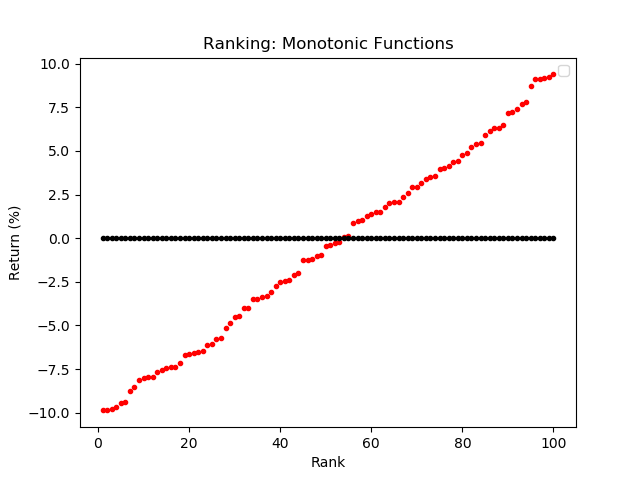
\includegraphics[width=\textwidth]{{/Users/connor/Google Drive/Documents/University/Courses/2020-21/Finance 788/finance-honours/results/plots/monotonic-ranking}.png}
    \caption{Monotonic ranking functions}
    \label{fig:mrf}
\end{figure}
First, we explore a ranking function with weights directly proportional to returns (\ref{w1})
to derive the below loss function (\ref{lf}).
\begin{align}
	R(\hat{y}) &= W \label{w1}\\
	W&:= \frac{\hat{y}}{\vec{\textbf{1}}\hat{y}}\\
	\hat{y} &= X^{T} \hat{\theta}\\
	f_{\hat{\theta}}(X) &= (\frac{X^{T} \hat{\theta}}{\vec{\textbf{1}}X^{T} \hat{\theta}})^\top X^{T} \hat{\theta} \label{lf}\\
\end{align}
Section \ref{sec:mlo} explains the theory on predicative modelling, loss functions and optimisation algorithms.
The ability to find partial derivatives (\ref{pdlf}) and argmax (\ref{argmax}) inform the practicality of this ranking function.
\begin{align}
	\frac{\partial f_{\hat{\theta}}(X)}{\partial \hat{\theta}} &= \frac{\partial ((\frac{X^{T} \hat{\theta}}{\vec{\textbf{1}}X^{T} \hat{\theta}})^\top X^{T} \hat{\theta})}{\partial \hat{\theta}} \label{pdlf}\\
	\argmax_{\hat{\theta}} &: (\frac{X^{T} \hat{\theta}}{\vec{\textbf{1}}X^{T} \hat{\theta}})^\top X^{T} \hat{\theta} \label{argmax}
\end{align}
The argmax (\label{argmax}) requires to use partial derivative with respect to $\hat{\theta}$
\begin{align}
	\frac{\partial (f_{\hat{\theta}}(X))}{\partial \hat{\theta}}  &= \frac{1}{(\hat{\theta}^\top X \vec{1})} X X^\top \hat{\theta}\\
	&+\frac{1}{\vec{1}X^\top \hat{\theta}} XX^\top \hat{\theta}\\
	&-\frac{1}{(\hat{\theta}^\top X \vec{1})^{2}} \hat{\theta}^\top XX^\top \hat{\theta} X \vec{1}
\end{align}
Subsequently, this enables the derivation of objective functions ex-post transaction costs.
\subsection{Optimisation of Hedge Portfolios}
Table \ref{hpt} provides a simple 
	\begin{table}[H]
		\centering
		\begin{tabular}{||c|c|c|c||}
			\hline
			Variable & Description & $ MSE(y,\hat{y}) $ & $ HP(y,\hat{y}) $\\ [0.5ex]
			\hline
			&&&\\
			$\theta$ & Est/Train& $ \hat{\theta}_{MSE}$& $ \hat{\theta}_{HP}$ \\ [0.5ex]
			\hline
			&&&\\
			$\lambda$ & Validation & $\hat{\lambda}_{MSE}$ & $\hat{\lambda}_{HP}$\\ [1.0ex]
			\hline
		\end{tabular}
	\caption{Objective (MSE: Mean Square Error, HP: Hedge Portfolio)}
	\label{hpt}
\end{table}
\newpage

\section{Data}
\textbf{Expand: Dataset implies, use this dataset (\cite{jensen2021there})}
Hou et al., (\citeyear{hou2020replicating}) use an extensive data library to assess 452 anomalies across anomalies literature.
Their analysis informs which abnormalities drive the cross section of expected returns. 
Most abnormalities fail under current standards of empirical finance when using a single hurdle test of absolute t-stat greater or equal to 1.96.
Firstly, the paper finds economic fundamentals take precedence over trading frictions in explanatory power, statistical and economic significance.
Secondly, micro-caps account for anomalies disproportionately, leading to NYSE breakpoints, value-weighted returns in both portfolio sorts and cross-sectional regressions with weighted least squares. 
Lastly, arguments in improving anomalies literature credibility follow a closer alignment to economic theory as the field persists to be statistical in nature.
Overall, capital market efficiency is higher than expected.
Jensen et al., \citeyear{jensen2021there} use the above dataset to explore hierarchial bayesian models of alphas emphasising the joint behaviours of factors, 
and provide an alternative multiple testing adjustment, more powerful than common methods.
Jensen et al., adapt the global dataset to focus only on one-month holding periods for all factors, only include most recent accounting data (quarterly or annually) and add 15 new factors.
The exhaustive nature and accessibility of the global dataset makes it well-suited for exploring optimisation functions in neural-network construction.
\subsection{Summary Statistics}
\section{Methodology}
\textbf{Adapt for the context of this research essay}
\subsection{Project organisation}
GOCPI adopted Data Science best practice, as described by Wilson et al \cite{J:10}. Although these practices are
mostly reserved for data science projects, their principles are suitable for product development and version control. All data and
results were saved regularly and reproducible. The retention of data in all forms received high levels of attention. Project files were synched
continuously to Google Drive \cite{Google_Drive}. Git \cite{Git} was used to manage version control for GOCPI's source code, data, documentation and results.
Git stores a complete history of versions using Git hashes. These hashes are strings unique to each state of the
publicly available GOCPI repository\footnote[1]{https://github.com/CMCD1996/GOCPI}. Git hashes enabled the discretisation of GOCPI's development over time,
enabling the accessibility and recollection of all previous states given a unique git hash. This functionality
enabled reproducibility, error correction and the ability to revert to previous models.

\subsubsection{Version Control}\label{Version Control}
Git, hosted by GitHub, provided a comprehensive set of version control technologies. These technologies provided a range of benefits.
Firstly, Git is excellent at providing and supporting collaborative functionalities. The master version of a project is accessible for all
who have access to the repository. Each contributor could create custom copies of branches through pull requests on the master branch. Contributors
could commit changes to custom branches and push these changes to the master branch through push requests. The product manager could review these push requests,
approving suitable requests to integrate changes to the master branch. Collaborative efforts were possible with
commit messages describing the contributions from each contributor. This project had one contributor. Git ensured the histories of code, work and authors are stored.
The descriptive nature of the commit log ensured an accurate journal is kept.

\subsubsection{Folder Structure}
GOCPI maintained the file folder structure recommended in Wilson et al \cite{J:10}. 
Project organisation was paramount as the modelling of energy systems involves integrating a range of optimisation models, data files and documents. 
Wilson et al's recommendations were appropriate as data science projects require similar organisational rigor. 
Subsequently, file management and structure was most efficient and comprehensive. \textbf{GOCPI} is the root directory of this project and contains several sub directories: bin, data, doc, src and results.  
The \textbf{bin} sub directory contained external scripts and compiled programmes related to the GOCPI project. 
The \textbf{data} sub directory contained all raw data associated with the project. 
This data included energy statistics, energy balance datasets, partitioned geographies, standardised optimisation models and TIMES modelling frameworks.
The \textbf{doc} sub directory stored GOCPI's user guides, academic resources, research reports and project deliverables.
The \textbf{results} sub directory contained the output from optimisation simulations and processed data to display on dashboards and websites to inform investment and policy decisions.
The \textbf{src} sub directory stores the source code for preparing raw data, partitioning sets of geographies with varying granularities and the GOCPI python package available to download using PyPI\footnote[2]{https://pypi.org/} and install using pip\footnote[3]{https://pypi.org/project/pip/}.
All files were continuously backed up using Google Drive.

\subsubsection{Python}\label{python}
Python 3.7 was the primary coding language for the GOCPI project. 
GOCPI's objective is to enable any user to design and model their own energy system to inform investment and policy decisions.
The intention is to empower users to discuss energy investment and policy decisions made by public and private parties.
Additionally, GOCPI intends to reduce misinformation regarding energy policies and help assess the feasibility of meeting the International Energy Agency's Sustainable Development Scenario \cite{IEA_WEM}.
Python is omnipresent, widespread in software development. 
Python's language design makes the language highly productive and simple to use. 
Python can hand off computationally straining tasks to C/C++ and has first-class integration capabilities with these two languages.
The language also has a very active and supportive community \cite{Python_Features}.
In addition, Python is the most popular coding language on the planet defined by the PYPL PopularitY of Programming Language Index. 
As at August 2020, Python had 31.59\% of all language tutorial search instances on Google \cite{PYPL_Pop}.
Python has many useful packages for creating the GOCPI package such as NumPy, Scikit-learn, os, csv and Pandas. 
Programming is quick due to Python's dynamic nature.
The language is also open-source with no cost.
Subsequently, Python was the best language to ensure the GOCPI model is accessible for many users to use and extend.

\subsubsection{Package Management}
The Anaconda package management platform for Python \cite{Anaconda} was the chosen coding environment.
Anaconda is a well defined, free platform with known versions of python packages such as matplotlib, numpy and pip.
The use of this environment ensured both reproducibility and consistency across infrastructure.
Although this project required no collaboration, the use of Anaconda will inform future developers on how to manage collaborative processes, especially for packages which are less well-maintained. Anaconda allows you to create custom environments which was necessary for creating scalable linear optimization problems to express energy systems.
Pip is Python's default package manager and is included in the Anaconda package. 
Pip was used to install and update packages for python not available on Anaconda such as twine and the custom GOCPI package developed for this project.

\subsubsection{Excel}
It is important users are comfortable with using the GOCPI model. 
Energy modelling can be quite complex. The modelling process must be transparent to inform users how to build their own models.
Excel is ubiquitous across academic and professional communities.
Excel's omnipotence makes the software well-suited for describing the components of the GNU Mathprog energy system model.
The \textbf{GOCPI OseMOSYS Structure.xlsx} file describes the sets, paramaters, constraints and objective function of a scalable energy system model.
The User may toggle statement sets, parameters and constraints to adjust the complexity of the model. 
The model file was imported to a text file.
However, data related to these energy systems was stored using Python dictionaries, lists and NumPy arrays.
This Python formulation was later transcribed to a text file.
Excel is best for two dimensional variables or data stored in Codd-Boyce relational databases \cite{CBNF}.
The majority of parameters in energy systems were three or more dimensions. 
Therefore, Excel was not suitable to store these parameters.
Python dictionaries, lists and NumPy arrays were preferred alternatives.

\subsubsection{IBM ILOG CPLEX Optimization}
The OseMOSYS methodology (see \ref{OseMOSYS}) translates energy systems into linear programming problems. 
A solver was required to optimise these user-defined energy systems.
The IBM ILOG Optimization Studio \cite{IBM_ILOG}, more commonly known as CPLEX, was chosen to be this solver.
CPLEX solves very large linear programming problems using the Barrier Interior-point method \cite{IPM} or primal/dual variants of the Simplex Method \cite{Simplex}.
GOCPI's user-defined energy systems could be scaled up to model very large systems, creating large linear programming problems.

The IBM ILOG CPLEX Optimization Studio has an interface with the Python language based on a C programming interface.
Subsequently, Python APIs were available to run the CPLEX solver when installed either locally or on a cloud service.
The python packages are \textbf{cplex} and \textbf{docplex}. The cplex package contains classes for accessing CPLEX for the Python programming language. 
The Cplex class is the most important class in this package as provides methods for creating, modifying, querying, or solving optimisation problems.
Docplex also enables the formulation of new linear programmes where one creates the model, defines the decision variables, sets the constraints and expresses the objective function.
The user uses docplex to solve the linear programme on a local solver. 
Alternatively, the model can be solved on a private cloud using Decision Optimisation on Cloud service through the provision of a service url and personal API key.
The CPLEX Python APIs were most attractive as provided the user with a powerful commercial solver in an accessible format.

There is a caveat to the use of the CPLEX solver. The IBM ILOG CPLEX Optimization Studio is commercial by nature and requires a license to use.
Fortunately IBM have the IBM Academic Initiative \cite{IBM_AI}, granting students access to commercial software for free.
This commercial nature creates accessibility issues for users who are not enrolled at an academic institution or can afford to pay for the software.
Accessibility issues caused by the need for commercial solvers must be addressed to enable the distribution of the GOCPI product.

\subsubsection{IBM Watson Machine Learning Service}
The IBM CPLEX Optimisation Cplex python API is suitable for smaller models that can be solved locally.
As the model increases in complexity, the docplex Python API did enable the ability to solve larger linear programmes.
Unfortunately, IBM phased out the docplex Python API by incorporating the Decision Optimisation on Cloud services into the IBM Watson Machine Learning cloud services \cite{IBM_WML}.
This change occurred during September 2020.
This service uses IBM Cloud to access assets through credentials, create model deployments in IBM's servers and execute jobs to solve models.
The model deployments must be Python-based models with jobs specifying a payloads containing input data and output formats.

\subsubsection{PyPI}\label{PyPI}
PyPI\footnote{https://pypi.org/} is the Python Package Index, a repository of software for the python programming language.
This repository helps you find and install software developed by the Python community who have decided to share their work.
The GOCPI package is distributed from this platform to enable as many as possible the ability to model their own energy systems to inform and question energy policy and investment.
Enter command: \textbf{pip install GOCPI} in the terminal to install the package using pip package management software.

\subsubsection{Code Style} \label{CS}
The GOCPI project was developed as the GOCPI package. All development code is organised within this package.
The PEP8 style for Python Code was the formatting style for development code \cite{PEP8}. 
All code was formatted with \textbf{yapf}, a formatter maintained by Google to format Python files.
Standardised formatting is important as makes the code easy to read, helps optimise the code and promotes consistency.
Docstrings and commenting were most important in documentation. A docstring is a Python inline comment. 
Each class and function has an unique docstring, a one sentence description of the function, inputs with data types and types of outputs.
The Google style docstring was most appropriate because of it's readability, ease to write and consistency with the Google Style Guide.
Additionally, automated documentation generators (\textbf{pdoc3, Sphinx} etc.) can parse this format to create documentation.
This self-consistent code style facilitated best practise maintenance and enabled reproducibility.

\subsubsection{Infrastructure}
GOCPI creates scalable energy system optimisation models with complexity size dependent.
Computations either took place locally on a 128 GB, four core Apple MacBook Pro or remotely using a cloud service. 

\subsection{Documentation}
The GOCPI project is well documented to keep an accurate record of key design decisions.
The commit history described in \ref{Version Control} was the most important form of document.
Other explicit documentation methods were applied to supplement this commit history. 
These methods, in addition to in-code documentation, include project updates and meeting minutes
nested within a project logbook.

\subsubsection{Project updates}
Project updates were recorded as itemized lists.
Each item is a brief description of the work completed during that day, week or month.
Items include, but are not limited to, completing GOCPI submodules, researching energy system statistics, building websites or writing sections of this research report.
These updates were pivotal to exploring new options, monitoring progress and making decisions to drive forward development. 
For example, the decision to adopt the OseMOSYS methodology in favour of the TIMES modelling methodology.
Project updates were transcribed to the project logbook held in this project's research compendium.

\subsubsection{Meeting minutes}
Project meetings took place for half an hour once a week. 
These meetings included discussions on energy markets, modelling methodologies, project progress and key design decisions.
The minutes from these meetings accompanies project updates in the project logbook nested within the research compendium.

\section{Results}

\section{Discussion}

\section{Conclusion}
\newpage
\section{Appendix}
\subsection{Tables and Charts}
\begin{table}[h!]
	\centering
	begin{tabular}{lrrrrrrrr}
	\toprule
	{} &     count &          mean &           std &           min &           25\% &           50\% &           75\% &           max \\
	\midrule
	Unnamed: 0              &  100000.0 &  4.999950e+04 &  2.886766e+04 &      0.000000 &  2.499975e+04 &  4.999950e+04 &  7.499925e+04 &  9.999900e+04 \\
	permno                  &  100000.0 &  1.048988e+04 &  2.887334e+02 &  10000.000000 &  1.023900e+04 &  1.048100e+04 &  1.075100e+04 &  1.099800e+04 \\
	permco                  &  100000.0 &  1.026687e+04 &  5.756027e+03 &     13.000000 &  8.179000e+03 &  8.473000e+03 &  8.786000e+03 &  5.345600e+04 \\
	crsp\_shrcd              &  100000.0 &  1.086098e+01 &  3.614896e-01 &     10.000000 &  1.100000e+01 &  1.100000e+01 &  1.100000e+01 &  1.200000e+01 \\
	crsp\_exchcd             &  100000.0 &  2.506350e+00 &  8.401826e-01 &      1.000000 &  2.000000e+00 &  3.000000e+00 &  3.000000e+00 &  3.000000e+00 \\
	sic                     &   99587.0 &  4.933514e+03 &  1.790397e+03 &    100.000000 &  3.541000e+03 &  4.955000e+03 &  6.324000e+03 &  9.997000e+03 \\
	ff49                    &   99337.0 &  3.189945e+01 &  1.438264e+01 &      1.000000 &  1.800000e+01 &  3.600000e+01 &  4.500000e+01 &  4.900000e+01 \\
	adjfct                  &  100000.0 &  2.378531e+00 &  1.061822e+01 &      0.003333 &  1.000000e+00 &  1.000000e+00 &  1.500000e+00 &  3.240000e+02 \\
	shares                  &  100000.0 &  7.500610e+01 &  5.179662e+02 &      0.236000 &  3.474000e+00 &  7.747000e+00 &  2.186800e+01 &  1.088022e+04 \\
	me                      &  100000.0 &  2.769919e+03 &  2.851385e+04 &      1.198969 &  2.649544e+01 &  8.089058e+01 &  3.639356e+02 &  1.706733e+06 \\
	me\_company              &  100000.0 &  2.786556e+03 &  2.859709e+04 &      1.198969 &  2.659784e+01 &  8.102900e+01 &  3.683085e+02 &  1.706733e+06 \\
	prc                     &  100000.0 &  2.075825e+01 &  3.837571e+01 &      0.046875 &  6.430000e+00 &  1.325000e+01 &  2.450000e+01 &  1.208800e+03 \\
	prc\_local               &  100000.0 &  2.075825e+01 &  3.837571e+01 &      0.046875 &  6.430000e+00 &  1.325000e+01 &  2.450000e+01 &  1.208800e+03 \\
	dolvol                  &   98694.0 &  2.924115e+08 &  2.828201e+09 &      0.000000 &  4.550000e+05 &  2.514414e+06 &  1.894224e+07 &  2.539520e+11 \\
	ret                     &   99317.0 &  1.616719e-02 &  1.636523e-01 &     -1.000000 & -5.769231e-02 &  0.000000e+00 &  7.178751e-02 &  6.000000e+00 \\
	ret\_local               &   99317.0 &  1.616719e-02 &  1.636523e-01 &     -1.000000 & -5.769231e-02 &  0.000000e+00 &  7.178751e-02 &  6.000000e+00 \\
	ret\_exc                 &   99317.0 &  1.224024e-02 &  1.637368e-01 &     -1.006810 & -6.171986e-02 & -2.286000e-03 &  6.824456e-02 &  5.996506e+00 \\
	ret\_lag\_dif             &  100000.0 &  1.000000e+00 &  0.000000e+00 &      1.000000 &  1.000000e+00 &  1.000000e+00 &  1.000000e+00 &  1.000000e+00 \\
	ret\_exc\_lead1m          &   99804.0 &  5.166515e-03 &  1.547285e-01 &     -1.006810 & -6.513292e-02 & -3.366000e-03 &  6.428314e-02 &  5.556758e+00 \\
	market\_equity\_rank\_x    &  100000.0 &  5.523121e+01 &  2.424970e+01 &      1.000000 &  3.500000e+01 &  5.300000e+01 &  7.500000e+01 &  9.950000e+01 \\
	enterprise\_value\_rank\_x &   83158.0 &  5.515533e+01 &  2.555834e+01 &      1.000000 &  3.400000e+01 &  5.400000e+01 &  7.700000e+01 &  9.950000e+01 \\
	book\_equity\_rank\_x      &   82123.0 &  5.437743e+01 &  2.705865e+01 &      1.000000 &  3.300000e+01 &  5.300000e+01 &  7.800000e+01 &  9.950000e+01 \\
	assets\_rank\_x           &   84556.0 &  5.565904e+01 &  2.753505e+01 &      1.000000 &  3.200000e+01 &  5.700000e+01 &  8.100000e+01 &  9.950000e+01 \\
	sales\_rank\_x            &   83650.0 &  5.447612e+01 &  2.711683e+01 &      1.000000 &  3.300000e+01 &  5.400000e+01 &  7.800000e+01 &  9.950000e+01 \\
	net\_income\_rank\_x       &   84299.0 &  5.497000e+01 &  2.791229e+01 &      1.000000 &  3.500000e+01 &  5.700000e+01 &  7.700000e+01 &  9.950000e+01 \\
	bidask\_x                &  100000.0 &  1.671600e-01 &  3.731205e-01 &      0.000000 &  0.000000e+00 &  0.000000e+00 &  0.000000e+00 &  1.000000e+00 \\
	prc\_high\_x              &   81488.0 &  2.296097e+01 &  2.491060e+01 &      0.281250 &  8.500000e+00 &  1.600000e+01 &  2.900000e+01 &  4.617600e+02 \\
	prc\_low\_x               &   82252.0 &  2.005462e+01 &  2.231967e+01 &      0.125000 &  7.000000e+00 &  1.375000e+01 &  2.537500e+01 &  4.175300e+02 \\
	tvol\_x                  &   98694.0 &  5.526569e+06 &  2.716632e+07 &      0.000000 &  5.475000e+04 &  2.354500e+05 &  1.192538e+06 &  6.485186e+08 \\
	div1m\_me\_x              &   99301.0 &  1.141127e-03 &  3.373808e-03 &      0.000000 &  0.000000e+00 &  0.000000e+00 &  0.000000e+00 &  9.013069e-02 \\
	div3m\_me\_x              &   99304.0 &  3.455602e-03 &  5.471153e-03 &      0.000000 &  0.000000e+00 &  0.000000e+00 &  6.153847e-03 &  1.164144e-01 \\
	div6m\_me\_x              &   97406.0 &  7.102777e-03 &  1.075952e-02 &      0.000000 &  0.000000e+00 &  0.000000e+00 &  1.249471e-02 &  1.350614e-01 \\
	div12m\_me\_x             &   93771.0 &  1.479920e-02 &  2.206019e-02 &      0.000000 &  0.000000e+00 &  0.000000e+00 &  2.555536e-02 &  2.853118e-01 \\
	chcsho\_1m\_x             &   99362.0 &  3.212910e-03 &  2.676977e-02 &     -0.116815 &  0.000000e+00 &  0.000000e+00 &  0.000000e+00 &  6.996410e-01 \\
	chcsho\_3m\_x             &   98093.0 &  1.231348e-02 &  6.122738e-02 &     -0.139411 &  0.000000e+00 &  0.000000e+00 &  3.277829e-03 &  1.238208e+00 \\
	chcsho\_6m\_x             &   96210.0 &  2.751299e-02 &  1.126550e-01 &     -0.176346 &  0.000000e+00 &  9.251229e-04 &  1.032486e-02 &  2.803931e+00 \\
	chcsho\_12m\_x            &   92666.0 &  6.148052e-02 &  2.132606e-01 &     -0.263229 &  0.000000e+00 &  4.452926e-03 &  3.278419e-02 &  4.162894e+00 \\
	eqnpo\_1m\_x              &   99300.0 & -1.599063e-03 &  2.398460e-02 &     -0.530417 & -2.953366e-09 &  0.000000e+00 &  3.239383e-09 &  1.263216e-01 \\
	eqnpo\_3m\_x              &   97944.0 & -6.543032e-03 &  5.216505e-02 &     -0.805667 & -1.875397e-03 &  1.963876e-09 &  7.120885e-03 &  1.682730e-01 \\
	eqnpo\_6m\_x              &   95942.0 & -1.386052e-02 &  8.761607e-02 &     -1.336026 & -7.228694e-03 &  2.267332e-09 &  1.492514e-02 &  2.787605e-01 \\
	eqnpo\_12m\_x             &   92243.0 & -2.812979e-02 &  1.463166e-01 &     -1.641488 & -2.469933e-02 &  3.605147e-10 &  3.115955e-02 &  4.742966e-01 \\
	ret\_1\_0\_x               &   89880.0 &  1.469405e-02 &  1.481324e-01 &     -0.702586 & -6.186453e-02 &  7.633630e-03 &  7.662956e-02 &  2.176471e+00 \\
	ret\_2\_0\_x               &   89196.0 &  2.926343e-02 &  2.110165e-01 &     -0.784206 & -8.078757e-02 &  1.340826e-02 &  1.154936e-01 &  3.342466e+00 \\
	ret\_3\_0\_x               &   88594.0 &  4.348828e-02 &  2.619169e-01 &     -0.874142 & -9.540903e-02 &  2.097522e-02 &  1.498982e-01 &  5.000000e+00 \\
	ret\_3\_1\_x               &   88575.0 &  2.853413e-02 &  2.094853e-01 &     -0.812500 & -8.100121e-02 &  1.304348e-02 &  1.153619e-01 &  3.342466e+00 \\
	ret\_6\_0\_x               &   86806.0 &  8.693332e-02 &  3.876104e-01 &     -0.911980 & -1.268082e-01 &  4.294117e-02 &  2.324574e-01 &  8.555556e+00 \\
	ret\_6\_1\_x               &   86754.0 &  7.169911e-02 &  3.479608e-01 &     -0.917098 & -1.180619e-01 &  3.498405e-02 &  2.051282e-01 &  8.411765e+00 \\
	ret\_9\_0\_x               &   85134.0 &  1.287106e-01 &  4.928214e-01 &     -0.967262 & -1.497804e-01 &  6.174438e-02 &  3.046733e-01 &  9.857143e+00 \\
	ret\_9\_1\_x               &   85025.0 &  1.137905e-01 &  4.565818e-01 &     -0.945833 & -1.431280e-01 &  5.555556e-02 &  2.798518e-01 &  9.273728e+00 \\
	ret\_12\_0\_x              &   83458.0 &  1.749940e-01 &  6.032653e-01 &     -0.960000 & -1.656086e-01 &  7.954546e-02 &  3.732819e-01 &  1.301592e+01 \\
	ret\_12\_1\_x              &   83348.0 &  1.574835e-01 &  5.624462e-01 &     -0.972763 & -1.604938e-01 &  7.229982e-02 &  3.477658e-01 &  1.223077e+01 \\
	ret\_12\_7\_x              &   83314.0 &  6.937836e-02 &  3.404595e-01 &     -0.875000 & -1.173493e-01 &  3.287172e-02 &  2.000000e-01 &  8.509434e+00 \\
	ret\_18\_1\_x              &   80200.0 &  2.556601e-01 &  7.712462e-01 &     -0.970071 & -1.824084e-01 &  1.150380e-01 &  4.910667e-01 &  2.048485e+01 \\
	ret\_24\_1\_x              &   77210.0 &  3.561783e-01 &  9.326939e-01 &     -0.964844 & -1.860465e-01 &  1.636364e-01 &  6.200000e-01 &  1.484615e+01 \\
	ret\_24\_12\_x             &   77107.0 &  1.716182e-01 &  5.903369e-01 &     -0.952381 & -1.594150e-01 &  7.673844e-02 &  3.601719e-01 &  1.345161e+01 \\
	ret\_36\_1\_x              &   71757.0 &  5.782320e-01 &  1.299369e+00 &     -0.984514 & -1.761381e-01 &  2.776960e-01 &  8.842902e-01 &  1.914000e+01 \\
	ret\_36\_12\_x             &   71493.0 &  3.769656e-01 &  9.657810e-01 &     -0.962121 & -1.750000e-01 &  1.731688e-01 &  6.308270e-01 &  1.508065e+01 \\
	ret\_48\_12\_x             &   66152.0 &  5.972792e-01 &  1.313366e+00 &     -0.983600 & -1.560323e-01 &  2.927964e-01 &  8.965517e-01 &  1.811811e+01 \\
	ret\_48\_1\_x              &   66379.0 &  8.118091e-01 &  1.618954e+00 &     -0.991708 & -1.384253e-01 &  4.097705e-01 &  1.182080e+00 &  1.641714e+01 \\
	ret\_60\_1\_x              &   61417.0 &  1.094750e+00 &  2.041543e+00 &     -0.995389 & -6.468322e-02 &  5.770103e-01 &  1.500000e+00 &  2.754724e+01 \\
	ret\_60\_12\_x             &   61101.0 &  8.308102e-01 &  1.638511e+00 &     -0.993829 & -1.125176e-01 &  4.304058e-01 &  1.185482e+00 &  1.791406e+01 \\
	ret\_60\_36\_x             &   60690.0 &  3.719123e-01 &  9.320425e-01 &     -0.957597 & -1.604938e-01 &  1.803905e-01 &  6.216216e-01 &  1.645517e+01 \\
	seas\_1\_1an\_x            &   87816.0 &  1.410007e-02 &  1.435859e-01 &     -0.670455 & -6.122449e-02 &  7.142857e-03 &  7.549050e-02 &  1.823529e+00 \\
	seas\_1\_1na\_x            &   59424.0 &  1.527346e-02 &  4.271727e-02 &     -0.215256 & -7.413571e-03 &  1.271693e-02 &  3.474624e-02 &  3.871171e-01 \\
	seas\_2\_5an\_x            &   56641.0 &  1.519025e-02 &  7.040538e-02 &     -0.293678 & -2.370873e-02 &  1.104103e-02 &  4.825217e-02 &  6.337087e-01 \\
	at\_gr1\_x                &   79717.0 &  2.340090e-01 &  6.237099e-01 &     -0.682279 &  4.476727e-03 &  8.921103e-02 &  2.391071e-01 &  1.032567e+01 \\
	ca\_gr1\_x                &   68947.0 &  2.849555e-01 &  9.986195e-01 &     -0.821969 & -4.250543e-02 &  9.021184e-02 &  2.847380e-01 &  1.567901e+01 \\
	nca\_gr1\_x               &   68931.0 &  3.417156e-01 &  1.099975e+00 &     -0.795148 & -2.000294e-02 &  8.607418e-02 &  2.985666e-01 &  2.841418e+01 \\
	lt\_gr1\_x                &   79185.0 &  2.939437e-01 &  9.534352e-01 &     -0.802141 & -3.323645e-02 &  8.336500e-02 &  2.805315e-01 &  1.384379e+01 \\
	cl\_gr1\_x                &   69011.0 &  2.962150e-01 &  9.203348e-01 &     -0.849398 & -7.455677e-02 &  1.039493e-01 &  3.647487e-01 &  1.258459e+01 \\
	ncl\_gr1\_x               &   64456.0 &  1.020352e+00 &  5.140075e+00 &     -1.000000 & -1.234226e-01 &  2.977931e-02 &  3.278159e-01 &  1.000349e+02 \\
	be\_gr1\_x                &   76414.0 &  3.229573e-01 &  1.169552e+00 &     -0.916605 &  9.176165e-03 &  9.628670e-02 &  2.341683e-01 &  2.281264e+01 \\
	debt\_gr1\_x              &   70167.0 &  7.568517e-01 &  4.078033e+00 &     -1.000000 & -1.544372e-01 &  1.505383e-02 &  3.400684e-01 &  1.028462e+02 \\
	sale\_gr1\_x              &   78017.0 &  2.150658e-01 &  6.419372e-01 &     -0.916926 &  6.138170e-04 &  1.028502e-01 &  2.500313e-01 &  1.370567e+01 \\
	cogs\_gr1\_x              &   77838.0 &  2.007377e-01 &  5.683719e-01 &     -0.959409 & -1.055398e-02 &  1.028721e-01 &  2.650250e-01 &  9.100222e+00 \\
	sga\_gr1\_x               &   64077.0 &  1.752823e-01 &  3.541695e-01 &     -0.619202 &  1.661077e-02 &  1.017764e-01 &  2.356600e-01 &  6.424410e+00 \\
	opex\_gr1\_x              &   77979.0 &  1.822789e-01 &  4.163107e-01 &     -0.766837 &  4.384702e-03 &  1.054838e-01 &  2.501507e-01 &  7.187355e+00 \\
	capx\_gr1\_x              &   68877.0 &  6.869989e-01 &  2.476468e+00 &     -1.336969 & -2.551566e-01 &  1.093750e-01 &  6.662180e-01 &  3.425000e+01 \\
	inv\_gr1\_x               &   64936.0 &  2.967757e-01 &  1.134464e+00 &     -1.000000 & -9.695228e-02 &  7.954545e-02 &  3.245350e-01 &  1.698084e+01 \\
	at\_gr3\_x                &   68888.0 &  7.703188e-01 &  1.636661e+00 &     -0.879679 &  8.189505e-02 &  3.294655e-01 &  8.300190e-01 &  2.153401e+01 \\
	ca\_gr3\_x                &   59990.0 &  8.228253e-01 &  2.119427e+00 &     -0.909899 &  1.107900e-02 &  3.049346e-01 &  8.473189e-01 &  3.133333e+01 \\
	nca\_gr3\_x               &   59997.0 &  1.289564e+00 &  4.052545e+00 &     -0.925747 &  3.869653e-02 &  3.478378e-01 &  1.052338e+00 &  1.752574e+02 \\
	lt\_gr3\_x                &   68299.0 &  1.031757e+00 &  2.895572e+00 &     -0.893593 &  3.261397e-02 &  3.369091e-01 &  9.355124e-01 &  4.643665e+01 \\
	cl\_gr3\_x                &   59905.0 &  9.406877e-01 &  2.564040e+00 &     -0.919418 & -7.453152e-03 &  3.546168e-01 &  9.877497e-01 &  3.934854e+01 \\
	ncl\_gr3\_x               &   55807.0 &  4.049907e+00 &  1.924271e+01 &     -1.000000 & -1.549412e-01 &  2.622823e-01 &  1.301106e+00 &  5.736961e+02 \\
	be\_gr3\_x                &   65580.0 &  9.686404e-01 &  2.750482e+00 &     -0.927249 &  6.973478e-02 &  3.140574e-01 &  8.430556e-01 &  6.185919e+01 \\
	debt\_gr3\_x              &   60299.0 &  3.042406e+00 &  1.514340e+01 &     -1.000000 & -2.407629e-01 &  2.125217e-01 &  1.182724e+00 &  4.269775e+02 \\
	sale\_gr3\_x              &   67321.0 &  8.305787e-01 &  2.444764e+00 &     -0.993046 &  6.950777e-02 &  3.284109e-01 &  7.885896e-01 &  5.854740e+01 \\
	cogs\_gr3\_x              &   66844.0 &  7.254693e-01 &  1.799863e+00 &     -0.975038 &  4.049441e-02 &  3.284997e-01 &  8.118149e-01 &  2.624880e+01 \\
	sga\_gr3\_x               &   54237.0 &  6.196393e-01 &  1.101842e+00 &     -0.820593 &  1.060271e-01 &  3.421648e-01 &  7.491501e-01 &  1.877127e+01 \\
	opex\_gr3\_x              &   66963.0 &  6.635705e-01 &  1.401121e+00 &     -0.897948 &  7.536986e-02 &  3.378616e-01 &  7.728895e-01 &  1.909844e+01 \\
	capx\_gr3\_x              &   59309.0 &  1.762974e+00 &  6.205317e+00 &     -1.208835 & -2.642717e-01 &  3.108488e-01 &  1.366906e+00 &  1.076800e+02 \\
	cash\_gr1a\_x             &   78604.0 &  1.135718e-02 &  1.375410e-01 &     -1.128632 & -1.659912e-02 &  2.359835e-03 &  3.347940e-02 &  8.302618e-01 \\
	inv\_gr1a\_x              &   77556.0 &  1.217829e-02 &  5.766522e-02 &     -0.372305 & -1.600734e-03 &  7.202984e-04 &  2.453485e-02 &  2.926627e-01 \\
	rec\_gr1a\_x              &   77779.0 &  2.543997e-02 &  7.279079e-02 &     -0.418567 & -3.799109e-03 &  1.516738e-02 &  4.976370e-02 &  3.340411e-01 \\
	ppeg\_gr1a\_x             &   68712.0 &  4.788804e-02 &  9.573047e-02 &     -0.729515 &  8.773603e-03 &  3.485520e-02 &  7.680075e-02 &  5.541908e-01 \\
	lti\_gr1a\_x              &   73504.0 &  7.220756e-03 &  4.863868e-02 &     -0.496427 &  0.000000e+00 &  0.000000e+00 &  2.234346e-03 &  3.477723e-01 \\
	intan\_gr1a\_x            &   67340.0 &  1.029751e-02 &  5.742975e-02 &     -0.761039 & -5.794232e-04 &  0.000000e+00 &  1.290345e-03 &  5.224851e-01 \\
	debtst\_gr1a\_x           &   78277.0 &  3.565424e-03 &  7.122081e-02 &     -0.523627 & -5.512812e-03 &  0.000000e+00 &  1.347066e-02 &  4.847275e-01 \\
	ap\_gr1a\_x               &   75016.0 &  1.658727e-02 &  5.520648e-02 &     -0.275446 & -5.126836e-03 &  7.247856e-03 &  3.049047e-02 &  2.944580e-01 \\
	txp\_gr1a\_x              &   65151.0 &  8.105253e-04 &  1.100964e-02 &     -0.068761 & -7.179940e-04 &  0.000000e+00 &  1.804448e-03 &  7.415345e-02 \\
	debtlt\_gr1a\_x           &   78853.0 &  1.703068e-02 &  1.017839e-01 &     -0.608519 & -1.123095e-02 &  0.000000e+00 &  3.326809e-02 &  5.760254e-01 \\
	txditc\_gr1a\_x           &   67398.0 &  1.984519e-03 &  1.132667e-02 &     -0.090702 &  0.000000e+00 &  0.000000e+00 &  3.895058e-03 &  8.328985e-02 \\
	coa\_gr1a\_x              &   68645.0 &  3.759837e-02 &  1.161911e-01 &     -0.790830 & -6.164059e-03 &  2.538175e-02 &  7.969422e-02 &  4.923150e-01 \\
	col\_gr1a\_x              &   69016.0 &  1.969095e-02 &  7.047457e-02 &     -0.470555 & -7.172744e-03 &  1.358034e-02 &  4.410158e-02 &  3.834478e-01 \\
	cowc\_gr1a\_x             &   67837.0 &  1.791927e-02 &  9.896435e-02 &     -0.605159 & -1.876779e-02 &  1.246806e-02 &  5.558615e-02 &  4.185010e-01 \\
	ncoa\_gr1a\_x             &   68947.0 &  4.753768e-02 &  1.315620e-01 &     -1.261411 & -6.706370e-03 &  2.793829e-02 &  8.686355e-02 &  7.493556e-01 \\
	ncol\_gr1a\_x             &   68383.0 &  6.431273e-03 &  3.271964e-02 &     -0.360464 & -9.663496e-04 &  6.525698e-04 &  1.052875e-02 &  3.337533e-01 \\
	nncoa\_gr1a\_x            &   67506.0 &  3.989812e-02 &  1.330547e-01 &     -1.232367 & -1.086804e-02 &  2.360237e-02 &  7.839400e-02 &  6.860888e-01 \\
	oa\_gr1a\_x               &   68645.0 &  8.497779e-02 &  2.036658e-01 &     -1.547159 & -5.319661e-03 &  6.883358e-02 &  1.712985e-01 &  8.015212e-01 \\
	ol\_gr1a\_x               &   68383.0 &  2.637089e-02 &  8.431216e-02 &     -0.574381 & -5.649730e-03 &  2.023225e-02 &  5.580244e-02 &  5.422407e-01 \\
	fna\_gr1a\_x              &   83531.0 &  5.850670e-03 &  5.818615e-02 &     -0.584246 &  0.000000e+00 &  0.000000e+00 &  0.000000e+00 &  6.895915e-01 \\
	fnl\_gr1a\_x              &   79044.0 &  2.087692e-02 &  1.273948e-01 &     -0.869471 & -1.671030e-02 &  0.000000e+00 &  5.263158e-02 &  9.213636e-01 \\
	nfna\_gr1a\_x             &   79044.0 & -1.476261e-02 &  1.473476e-01 &     -1.053214 & -5.615308e-02 &  0.000000e+00 &  2.727055e-02 &  9.020642e-01 \\
	gp\_gr1a\_x               &   77982.0 &  3.866234e-02 &  1.236833e-01 &     -0.745759 & -3.193912e-03 &  1.961027e-02 &  7.562234e-02 &  1.122939e+00 \\
	ebitda\_gr1a\_x           &   78132.0 &  9.893444e-03 &  9.809898e-02 &     -0.737330 & -1.159388e-02 &  8.472428e-03 &  4.009246e-02 &  1.186792e+00 \\
	ebit\_gr1a\_x             &   78113.0 &  5.169471e-03 &  9.696567e-02 &     -0.834222 & -1.480965e-02 &  5.912272e-03 &  3.394289e-02 &  8.838689e-01 \\
	ope\_gr1a\_x              &   65573.0 &  1.011649e-02 &  1.036873e-01 &     -0.722895 & -1.745909e-02 &  1.196690e-02 &  4.370402e-02 &  1.179166e+00 \\
	ni\_gr1a\_x               &   78871.0 &  8.268237e-04 &  1.214660e-01 &     -1.688863 & -1.414863e-02 &  3.230521e-03 &  2.481572e-02 &  1.146474e+00 \\
	nix\_gr1a\_x              &   78871.0 &  9.680542e-04 &  1.323251e-01 &     -1.854896 & -1.641065e-02 &  3.075140e-03 &  2.596931e-02 &  1.175522e+00 \\
	dp\_gr1a\_x               &   75959.0 &  4.429358e-03 &  1.326722e-02 &     -0.132077 & -2.364490e-05 &  2.403962e-03 &  8.104667e-03 &  1.919576e-01 \\
	fincf\_gr1a\_x            &   65320.0 &  1.275394e-02 &  2.625873e-01 &     -1.756601 & -5.917252e-02 &  2.667307e-03 &  8.008256e-02 &  1.485072e+00 \\
	ocf\_gr1a\_x              &   77023.0 & -1.386009e-03 &  1.592057e-01 &     -0.985635 & -4.469304e-02 &  2.010443e-03 &  4.770744e-02 &  1.151193e+00 \\
	fcf\_gr1a\_x              &   69491.0 & -8.766654e-03 &  1.894055e-01 &     -1.119445 & -6.649983e-02 & -8.450264e-04 &  5.686808e-02 &  1.202901e+00 \\
	nwc\_gr1a\_x              &   68139.0 &  2.678592e-02 &  1.841561e-01 &     -1.338601 & -2.918488e-02 &  1.851852e-02 &  8.239146e-02 &  8.712542e-01 \\
	eqnetis\_gr1a\_x          &   65430.0 &  9.671970e-03 &  2.131677e-01 &     -1.591969 & -1.142824e-02 &  0.000000e+00 &  1.593471e-02 &  1.207629e+00 \\
	dltnetis\_gr1a\_x         &   77415.0 & -3.375011e-03 &  1.291037e-01 &     -0.787435 & -2.300374e-02 &  0.000000e+00 &  1.893497e-02 &  7.003337e-01 \\
	dstnetis\_gr1a\_x         &   75808.0 &  2.495908e-04 &  1.069491e-01 &     -0.806337 & -1.192910e-02 &  0.000000e+00 &  1.996083e-02 &  7.197279e-01 \\
	dbnetis\_gr1a\_x          &   77452.0 & -3.235691e-03 &  1.759903e-01 &     -1.026894 & -4.054027e-02 &  0.000000e+00 &  4.235530e-02 &  1.017915e+00 \\
	netis\_gr1a\_x            &   65429.0 &  4.876631e-03 &  2.851635e-01 &     -1.836024 & -6.502422e-02 &  1.123007e-03 &  7.699574e-02 &  1.539881e+00 \\
	eqnpo\_gr1a\_x            &   65430.0 & -9.129002e-03 &  2.167009e-01 &     -1.182054 & -1.697817e-02 &  0.000000e+00 &  1.371429e-02 &  1.591969e+00 \\
	tax\_gr1a\_x              &   78222.0 &  2.549608e-03 &  2.769618e-02 &     -0.215707 & -4.079819e-03 &  7.975302e-04 &  1.060251e-02 &  1.883751e-01 \\
	eqbb\_gr1a\_x             &   60903.0 &  1.547406e-03 &  3.389438e-02 &     -0.380617 &  0.000000e+00 &  0.000000e+00 &  4.022115e-04 &  2.808763e-01 \\
	eqis\_gr1a\_x             &   62991.0 &  1.067099e-02 &  2.124967e-01 &     -1.584441 & -2.624568e-03 &  0.000000e+00 &  6.636662e-03 &  1.207629e+00 \\
	div\_gr1a\_x              &   77971.0 &  7.471557e-04 &  9.042162e-03 &     -0.218255 &  0.000000e+00 &  0.000000e+00 &  6.030800e-04 &  2.030233e-01 \\
	eqpo\_gr1a\_x             &   60903.0 &  2.427553e-03 &  4.216114e-02 &     -0.461986 & -1.137891e-04 &  0.000000e+00 &  3.646585e-03 &  3.901357e-01 \\
	capx\_gr1a\_x             &   69614.0 &  6.759772e-03 &  5.689882e-02 &     -0.417812 & -8.421897e-03 &  2.170374e-03 &  1.959634e-02 &  3.895335e-01 \\
	be\_gr1a\_x               &   76414.0 &  4.664042e-02 &  1.700975e-01 &     -1.543012 &  2.124536e-03 &  3.243210e-02 &  9.160714e-02 &  8.468710e-01 \\
	cash\_gr3a\_x             &   67841.0 &  2.272632e-02 &  1.845090e-01 &     -2.461024 & -1.487601e-02 &  8.141066e-03 &  6.231487e-02 &  7.963663e-01 \\
	inv\_gr3a\_x              &   66702.0 &  2.669011e-02 &  9.353412e-02 &     -0.687334 & -2.638247e-04 &  6.147909e-03 &  5.502052e-02 &  4.114685e-01 \\
	rec\_gr3a\_x              &   67104.0 &  5.819278e-02 &  1.204527e-01 &     -0.779534 &  3.438571e-03 &  3.961086e-02 &  1.080324e-01 &  4.875428e-01 \\
	ppeg\_gr3a\_x             &   59478.0 &  1.143134e-01 &  1.812052e-01 &     -1.655304 &  2.919725e-02 &  1.007662e-01 &  1.924517e-01 &  8.332787e-01 \\
	lti\_gr3a\_x              &   61945.0 &  1.707528e-02 &  8.515605e-02 &     -0.656623 &  0.000000e+00 &  0.000000e+00 &  1.275369e-02 &  4.683121e-01 \\
	intan\_gr3a\_x            &   56225.0 &  2.469689e-02 &  1.024489e-01 &     -1.793814 & -5.099699e-05 &  0.000000e+00 &  2.023025e-02 &  6.632143e-01 \\
	debtst\_gr3a\_x           &   67457.0 &  7.858057e-03 &  9.203482e-02 &     -0.831497 & -7.007479e-03 &  1.451193e-04 &  2.613803e-02 &  5.513702e-01 \\
	ap\_gr3a\_x               &   63589.0 &  3.990997e-02 &  9.499532e-02 &     -0.497308 & -6.118856e-04 &  1.878518e-02 &  5.864005e-02 &  4.738813e-01 \\
	txp\_gr3a\_x              &   55529.0 &  1.489925e-03 &  1.340925e-02 &     -0.076289 & -1.064963e-03 &  0.000000e+00 &  3.528661e-03 &  8.995905e-02 \\
	debtlt\_gr3a\_x           &   68086.0 &  3.678976e-02 &  1.560884e-01 &     -1.169989 & -1.297859e-02 &  8.776581e-03 &  9.143539e-02 &  7.496221e-01 \\
	txditc\_gr3a\_x           &   58233.0 &  5.085601e-03 &  2.056567e-02 &     -0.165240 &  0.000000e+00 &  0.000000e+00 &  1.026694e-02 &  1.072464e-01 \\
	coa\_gr3a\_x              &   59716.0 &  8.130334e-02 &  1.910139e-01 &     -1.441231 &  6.143018e-03 &  6.922210e-02 &  1.689665e-01 &  6.791055e-01 \\
	col\_gr3a\_x              &   59907.0 &  4.500265e-02 &  1.053162e-01 &     -0.965261 &  3.879323e-03 &  3.820093e-02 &  8.630953e-02 &  4.559172e-01 \\
	cowc\_gr3a\_x             &   58839.0 &  3.653286e-02 &  1.484395e-01 &     -1.040474 & -2.098227e-02 &  2.973004e-02 &  1.033972e-01 &  5.603979e-01 \\
	ncoa\_gr3a\_x             &   60007.0 &  1.050067e-01 &  2.306541e-01 &     -3.870719 &  9.087089e-03 &  9.623946e-02 &  2.117214e-01 &  8.086193e-01 \\
	ncol\_gr3a\_x             &   59211.0 &  1.598156e-02 &  5.947009e-02 &     -0.578248 & -6.920073e-05 &  5.999244e-03 &  2.592810e-02 &  3.988077e-01 \\
	nncoa\_gr3a\_x            &   58434.0 &  8.675169e-02 &  2.252497e-01 &     -3.194340 & -4.928137e-04 &  7.958930e-02 &  1.887284e-01 &  7.883821e-01 \\
	oa\_gr3a\_x               &   59716.0 &  1.854313e-01 &  3.556953e-01 &     -4.043893 &  4.026295e-02 &  2.014626e-01 &  3.832832e-01 &  9.247126e-01 \\
	ol\_gr3a\_x               &   59211.0 &  6.057444e-02 &  1.330810e-01 &     -0.974292 &  1.182179e-02 &  5.761910e-02 &  1.140134e-01 &  6.233345e-01 \\
	fna\_gr3a\_x              &   76568.0 &  1.697186e-02 &  9.083223e-02 &     -1.032585 &  0.000000e+00 &  0.000000e+00 &  0.000000e+00 &  6.829162e-01 \\
	fnl\_gr3a\_x              &   68310.0 &  4.619417e-02 &  1.989910e-01 &     -1.644118 & -1.874554e-02 &  2.297731e-02 &  1.244181e-01 &  8.753479e-01 \\
	nfna\_gr3a\_x             &   68310.0 & -3.360455e-02 &  2.211303e-01 &     -1.248189 & -1.249060e-01 & -1.872066e-02 &  4.427796e-02 &  1.644118e+00 \\
	gp\_gr3a\_x               &   66990.0 &  8.348589e-02 &  2.032856e-01 &     -1.128507 &  3.839957e-03 &  5.376685e-02 &  1.624814e-01 &  9.814586e-01 \\
	ebitda\_gr3a\_x           &   67269.0 &  2.247433e-02 &  1.361932e-01 &     -0.884279 & -1.071769e-02 &  2.151470e-02 &  7.452829e-02 &  1.271214e+00 \\
	ebit\_gr3a\_x             &   67236.0 &  1.189171e-02 &  1.345816e-01 &     -1.026774 & -1.766170e-02 &  1.392220e-02 &  5.929624e-02 &  1.373007e+00 \\
	ope\_gr3a\_x              &   56294.0 &  2.324199e-02 &  1.429630e-01 &     -0.841909 & -1.949482e-02 &  2.618806e-02 &  7.807622e-02 &  1.009807e+00 \\
	ni\_gr3a\_x               &   68031.0 &  3.280394e-03 &  1.486194e-01 &     -1.330393 & -1.722207e-02 &  6.743238e-03 &  4.072211e-02 &  1.217098e+00 \\
	nix\_gr3a\_x              &   68031.0 &  2.927618e-03 &  1.575718e-01 &     -1.271989 & -1.979606e-02 &  6.799154e-03 &  4.272763e-02 &  1.273113e+00 \\
	dp\_gr3a\_x               &   65031.0 &  1.054077e-02 &  2.405814e-02 &     -0.223649 &  4.545630e-04 &  7.301104e-03 &  1.922646e-02 &  2.037688e-01 \\
	ocf\_gr3a\_x              &   66200.0 &  2.196724e-02 &  1.675867e-01 &     -0.962350 & -3.143870e-02 &  1.281189e-02 &  7.549920e-02 &  1.459275e+00 \\
	fcf\_gr3a\_x              &   59801.0 &  1.434510e-02 &  1.944875e-01 &     -0.959419 & -6.064569e-02 &  7.450519e-03 &  7.650017e-02 &  1.662028e+00 \\
	nwc\_gr3a\_x              &   59130.0 &  5.304876e-02 &  2.553131e-01 &     -2.400334 & -2.829289e-02 &  5.008945e-02 &  1.613771e-01 &  9.098618e-01 \\
	dltnetis\_gr3a\_x         &   66766.0 & -8.454382e-03 &  1.395302e-01 &     -0.943679 & -2.863836e-02 &  0.000000e+00 &  1.901740e-02 &  8.602060e-01 \\
	dstnetis\_gr3a\_x         &   65151.0 & -1.455326e-03 &  9.284288e-02 &     -0.777637 & -1.439239e-02 &  0.000000e+00 &  1.755369e-02 &  6.541406e-01 \\
	dbnetis\_gr3a\_x          &   66799.0 & -9.665979e-03 &  1.754118e-01 &     -1.243730 & -4.496743e-02 &  0.000000e+00 &  3.891492e-02 &  1.075731e+00 \\
	tax\_gr3a\_x              &   67418.0 &  4.685190e-03 &  3.529203e-02 &     -0.218962 & -5.200458e-03 &  1.998450e-03 &  1.733238e-02 &  1.809693e-01 \\
	div\_gr3a\_x              &   67107.0 &  1.920768e-03 &  1.210645e-02 &     -0.205875 &  0.000000e+00 &  0.000000e+00 &  2.522659e-03 &  1.810838e-01 \\
	capx\_gr3a\_x             &   59930.0 &  1.024212e-02 &  6.735920e-02 &     -0.596642 & -7.570922e-03 &  6.323187e-03 &  3.056904e-02 &  3.583062e-01 \\
	capx\_at\_x               &   74522.0 &  6.405274e-02 &  7.352952e-02 &     -0.030504 &  1.845855e-02 &  4.280397e-02 &  8.151096e-02 &  5.760933e-01 \\
	spi\_at\_x                &   80392.0 & -8.938327e-03 &  4.499022e-02 &     -1.176871 & -5.042731e-04 &  0.000000e+00 &  0.000000e+00 &  1.960574e-01 \\
	xido\_at\_x               &   84265.0 &  6.160027e-05 &  1.687795e-02 &     -0.260502 &  0.000000e+00 &  0.000000e+00 &  0.000000e+00 &  1.761674e-01 \\
	nri\_at\_x                &   80392.0 & -9.093377e-03 &  5.510842e-02 &     -1.533786 & -2.029198e-03 &  0.000000e+00 &  0.000000e+00 &  2.675198e-01 \\
	gp\_sale\_x               &   83302.0 &  1.192524e-01 &  2.161043e+00 &   -108.252336 &  1.975654e-01 &  3.261121e-01 &  4.984402e-01 &  9.722307e-01 \\
	ebitda\_sale\_x           &   83389.0 & -2.042675e-01 &  2.961699e+00 &   -143.688525 &  5.236953e-02 &  1.215018e-01 &  2.165036e-01 &  7.141322e-01 \\
	ebit\_sale\_x             &   83369.0 & -2.682005e-01 &  3.091808e+00 &   -146.737705 &  2.551892e-02 &  8.570296e-02 &  1.654666e-01 &  5.693628e-01 \\
	pi\_sale\_x               &   83439.0 & -3.124057e-01 &  3.309065e+00 &   -174.174781 &  7.337319e-03 &  7.007719e-02 &  1.426619e-01 &  6.559774e-01 \\
	ni\_sale\_x               &   83441.0 & -3.380056e-01 &  3.248960e+00 &   -174.174781 &  4.740297e-03 &  4.408514e-02 &  9.292270e-02 &  5.417515e-01 \\
	nix\_sale\_x              &   83411.0 & -3.430431e-01 &  3.293034e+00 &   -174.174781 &  3.671240e-03 &  4.456242e-02 &  9.560031e-02 &  6.243023e-01 \\
	ocf\_sale\_x              &   82361.0 & -2.834958e-01 &  2.706786e+00 &   -115.470103 & -1.709783e-02 &  5.755859e-02 &  1.375354e-01 &  1.197232e+00 \\
	fcf\_sale\_x              &   74144.0 & -4.568814e-01 &  3.084399e+00 &   -114.804688 & -1.034250e-01 & -2.376246e-03 &  6.329335e-02 &  1.014327e+00 \\
	gp\_at\_x                 &   83519.0 &  3.058489e-01 &  3.075106e-01 &     -1.039113 &  7.776304e-02 &  2.762770e-01 &  4.781763e-01 &  1.412338e+00 \\
	ebitda\_at\_x             &   83606.0 &  7.254892e-02 &  1.964921e-01 &     -1.871416 &  2.402509e-02 &  1.025681e-01 &  1.681772e-01 &  4.597082e-01 \\
	ebit\_at\_x               &   83582.0 &  3.641471e-02 &  1.965754e-01 &     -1.910124 &  1.701226e-02 &  6.710267e-02 &  1.235551e-01 &  4.105165e-01 \\
	fi\_at\_x                 &   70643.0 &  1.285423e-02 &  2.116006e-01 &     -2.281424 &  1.815834e-02 &  6.301707e-02 &  9.733451e-02 &  3.715535e-01 \\
	cop\_at\_x                &   71079.0 &  1.242040e-01 &  2.137309e-01 &     -1.188215 &  3.174832e-02 &  1.325974e-01 &  2.364487e-01 &  1.531592e+00 \\
	ni\_at\_x                 &   84295.0 & -6.934733e-03 &  1.972960e-01 &     -2.300792 &  3.028539e-03 &  3.230118e-02 &  7.146967e-02 &  3.331630e-01 \\
	ope\_be\_x                &   68080.0 &  1.244371e-01 &  6.129974e-01 &     -8.379530 &  8.509552e-02 &  2.109810e-01 &  3.171122e-01 &  3.284896e+00 \\
	ni\_be\_x                 &   81843.0 & -4.170810e-02 &  6.540741e-01 &    -10.754148 &  1.944193e-02 &  9.476066e-02 &  1.466488e-01 &  1.450547e+00 \\
	nix\_be\_x                &   81843.0 & -4.512749e-02 &  6.799785e-01 &    -11.951532 &  1.740826e-02 &  9.614812e-02 &  1.489557e-01 &  1.558275e+00 \\
	ocf\_be\_x                &   80045.0 &  9.325967e-03 &  6.544577e-01 &     -7.245926 & -3.761535e-02 &  1.144212e-01 &  2.205872e-01 &  4.068686e+00 \\
	fcf\_be\_x                &   71780.0 & -1.769148e-01 &  8.234297e-01 &     -9.895939 & -2.180495e-01 & -4.334297e-03 &  1.286074e-01 &  2.895115e+00 \\
	gp\_bev\_x                &   81261.0 &  6.877303e-01 &  1.192313e+00 &     -9.210272 &  2.270252e-01 &  4.805274e-01 &  8.840906e-01 &  1.753113e+01 \\
	ebitda\_bev\_x            &   81348.0 &  7.059743e-02 &  1.031921e+00 &    -28.063673 &  8.688913e-02 &  1.814286e-01 &  3.008124e-01 &  3.228898e+00 \\
	ebit\_bev\_x              &   81328.0 & -1.460347e-02 &  1.100053e+00 &    -35.603143 &  4.670120e-02 &  1.289825e-01 &  2.286745e-01 &  2.634083e+00 \\
	fi\_bev\_x                &   68875.0 & -8.077968e-02 &  1.109721e+00 &    -21.894597 &  3.656339e-02 &  9.945921e-02 &  1.674235e-01 &  2.202873e+00 \\
	cop\_bev\_x               &   69611.0 &  2.923736e-01 &  8.535565e-01 &     -5.537906 &  7.534899e-02 &  2.259287e-01 &  4.371082e-01 &  1.244377e+01 \\
	gp\_ppen\_x               &   82611.0 &  2.921862e+00 &  5.386306e+00 &   -130.538462 &  6.349292e-01 &  1.863453e+00 &  3.900439e+00 &  1.035052e+02 \\
	ebitda\_ppen\_x           &   82698.0 &  5.588297e-01 &  5.310174e+00 &   -252.813559 &  2.015400e-01 &  5.743982e-01 &  1.387999e+00 &  3.389320e+01 \\
	fcf\_ppen\_x              &   73568.0 & -4.374453e-01 &  4.885994e+00 &   -229.500000 & -4.317279e-01 & -1.535052e-02 &  4.317829e-01 &  2.892105e+01 \\
	fincf\_at\_x              &   70465.0 &  5.923096e-02 &  2.276332e-01 &     -0.908497 & -3.863822e-02 &  1.868365e-03 &  8.381301e-02 &  1.539186e+00 \\
	netis\_at\_x              &   70522.0 &  2.586771e-02 &  2.588545e-01 &     -1.368065 & -4.814651e-02 & -7.912986e-04 &  5.578284e-02 &  1.430119e+00 \\
	eqnetis\_at\_x            &   70530.0 &  5.580960e-02 &  1.815813e-01 &     -0.350709 & -6.623314e-04 &  7.250965e-04 &  1.704739e-02 &  1.375146e+00 \\
	eqis\_at\_x               &   68765.0 &  7.020270e-02 &  1.843317e-01 &     -0.103400 &  7.457109e-05 &  3.428571e-03 &  2.609577e-02 &  1.407882e+00 \\
	dbnetis\_at\_x            &   82532.0 & -2.273721e-02 &  1.659351e-01 &     -1.362369 & -3.972132e-02 & -1.446212e-03 &  2.101781e-02 &  6.455704e-01 \\
	dltnetis\_at\_x           &   82512.0 & -2.416266e-02 &  1.381219e-01 &     -1.226849 & -3.050334e-02 & -3.224409e-03 &  0.000000e+00 &  5.183637e-01 \\
	dstnetis\_at\_x           &   81059.0 &  2.397359e-03 &  7.375303e-02 &     -0.478936 & -6.481128e-03 &  0.000000e+00 &  1.144933e-02 &  4.835838e-01 \\
	eqnpo\_at\_x              &   70530.0 & -4.684199e-02 &  1.858772e-01 &     -1.375146 & -1.352162e-02 &  0.000000e+00 &  1.557461e-02 &  4.461726e-01 \\
	eqbb\_at\_x               &   67111.0 &  1.170811e-02 &  3.229884e-02 &     -0.002558 &  0.000000e+00 &  0.000000e+00 &  5.502863e-03 &  4.017798e-01 \\
	div\_at\_x                &   83608.0 &  8.948964e-03 &  1.856573e-02 &      0.000000 &  0.000000e+00 &  0.000000e+00 &  1.006291e-02 &  2.644511e-01 \\
	oaccruals\_at\_x          &   71182.0 & -8.511955e-03 &  1.569651e-01 &     -2.004772 & -7.306808e-02 & -1.672894e-02 &  5.116442e-02 &  6.719221e-01 \\
	oaccruals\_ni\_x          &   71091.0 & -2.636272e-01 &  6.400549e+00 &    -71.441767 & -1.169122e+00 & -2.462554e-01 &  7.370952e-01 &  8.515789e+01 \\
	taccruals\_at\_x          &   70912.0 & -2.419045e-02 &  1.934654e-01 &     -2.276390 & -9.023051e-02 & -1.349768e-02 &  4.721009e-02 &  9.277600e-01 \\
	taccruals\_ni\_x          &   70803.0 & -1.038130e+00 &  7.895110e+00 &   -112.261538 & -1.439394e+00 & -2.018444e-01 &  7.259226e-01 &  6.728571e+01 \\
	noa\_at\_x                &   67827.0 &  6.624244e-01 &  4.239865e-01 &     -0.965822 &  4.576732e-01 &  6.774060e-01 &  8.305522e-01 &  4.265072e+00 \\
	be\_bev\_x                &   80358.0 &  1.337380e+00 &  2.313888e+00 &      0.035054 &  5.615100e-01 &  8.227822e-01 &  1.223881e+00 &  4.400549e+01 \\
	debt\_bev\_x              &   81603.0 &  4.635573e-01 &  5.203591e-01 &      0.000000 &  1.494456e-01 &  3.751129e-01 &  6.312745e-01 &  8.264789e+00 \\
	cash\_bev\_x              &   81239.0 &  8.065404e-01 &  2.594199e+00 &      0.000000 &  4.214693e-02 &  1.396889e-01 &  4.654783e-01 &  4.223059e+01 \\
	pstk\_bev\_x              &   82205.0 &  2.234662e-02 &  1.105032e-01 &      0.000000 &  0.000000e+00 &  0.000000e+00 &  0.000000e+00 &  2.730344e+00 \\
	debtlt\_bev\_x            &   81510.0 &  3.274546e-01 &  3.957937e-01 &      0.000000 &  4.695412e-02 &  2.499551e-01 &  4.585166e-01 &  6.674744e+00 \\
	debtst\_bev\_x            &   81109.0 &  1.303392e-01 &  2.386261e-01 &      0.000000 &  4.750627e-03 &  4.107521e-02 &  1.510107e-01 &  3.471524e+00 \\
	int\_debt\_x              &   62360.0 &  1.191078e-01 &  2.352767e-01 &      0.000000 &  5.559077e-02 &  7.925713e-02 &  1.098973e-01 &  7.543210e+00 \\
	int\_debtlt\_x            &   59223.0 &  3.477440e-01 &  1.333440e+00 &      0.000000 &  6.712647e-02 &  1.008625e-01 &  1.649806e-01 &  4.055319e+01 \\
	ebitda\_debt\_x           &   74454.0 &  1.873789e+00 &  1.369748e+01 &   -274.000000 &  1.469308e-01 &  4.032451e-01 &  9.404641e-01 &  3.095487e+02 \\
	profit\_cl\_x             &   72705.0 &  3.879935e-01 &  1.571841e+00 &    -11.903846 &  1.735159e-01 &  5.130435e-01 &  9.684604e-01 &  5.768146e+00 \\
	ocf\_cl\_x                &   72652.0 &  2.827570e-03 &  1.599381e+00 &    -14.956800 & -1.503859e-01 &  1.980802e-01 &  5.943197e-01 &  5.976386e+00 \\
	ocf\_debt\_x              &   73489.0 &  9.986423e-01 &  1.210108e+01 &   -239.354167 & -6.991422e-02 &  1.465671e-01 &  5.342936e-01 &  3.818136e+02 \\
	cash\_lt\_x               &   83132.0 &  8.512404e-01 &  2.430332e+00 &      0.000000 &  3.751187e-02 &  1.177077e-01 &  5.170697e-01 &  2.990909e+01 \\
	inv\_act\_x               &   66454.0 &  2.857719e-01 &  2.312413e-01 &      0.000000 &  5.815148e-02 &  2.767750e-01 &  4.605285e-01 &  9.008857e-01 \\
	rec\_act\_x               &   66896.0 &  3.547460e-01 &  2.078579e-01 &      0.000000 &  2.060601e-01 &  3.440109e-01 &  4.788401e-01 &  9.356141e-01 \\
	debtst\_debt\_x           &   74143.0 &  3.130781e-01 &  3.238387e-01 &      0.000000 &  4.503603e-02 &  1.876543e-01 &  4.984650e-01 &  1.000000e+00 \\
	cl\_lt\_x                 &   72576.0 &  5.751892e-01 &  2.798983e-01 &      0.018302 &  3.451427e-01 &  5.657963e-01 &  8.274718e-01 &  1.000000e+00 \\
	debtlt\_debt\_x           &   74698.0 &  6.992906e-01 &  3.227056e-01 &      0.000000 &  5.209669e-01 &  8.281028e-01 &  9.650736e-01 &  1.000000e+00 \\
	lt\_ppen\_x               &   82539.0 &  1.646287e+01 &  3.672835e+01 &      0.082926 &  1.172060e+00 &  2.420959e+00 &  8.045524e+00 &  5.580774e+02 \\
	debtlt\_be\_x             &   81349.0 &  7.088002e-01 &  1.481488e+00 &      0.000000 &  3.016158e-02 &  2.803062e-01 &  6.947088e-01 &  2.225157e+01 \\
	opex\_at\_x               &   83519.0 &  9.681317e-01 &  7.838660e-01 &      0.015471 &  3.676639e-01 &  8.565324e-01 &  1.357200e+00 &  5.195711e+00 \\
	nwc\_at\_x                &   72102.0 &  2.993303e-01 &  2.430646e-01 &     -0.750746 &  1.286938e-01 &  2.842063e-01 &  4.563323e-01 &  9.547180e-01 \\
	debt\_at\_x               &   83900.0 &  2.204809e-01 &  2.014133e-01 &      0.000000 &  5.117692e-02 &  1.814944e-01 &  3.300031e-01 &  1.362951e+00 \\
	debt\_be\_x               &   81454.0 &  1.004806e+00 &  2.067362e+00 &      0.000000 &  1.040678e-01 &  4.318686e-01 &  1.007597e+00 &  3.440000e+01 \\
	ebit\_int\_x              &   64860.0 &  2.203736e+01 &  1.439395e+02 &  -2004.500000 &  1.009360e+00 &  4.227928e+00 &  1.064839e+01 &  3.302250e+03 \\
	inv\_days\_x              &   81141.0 &  9.016036e+01 &  1.504356e+02 &      0.000000 &  1.058337e+01 &  5.807602e+01 &  1.147962e+02 &  3.361770e+03 \\
	rec\_days\_x              &   81348.0 &  4.533771e+02 &  1.063423e+03 &      0.000000 &  4.095771e+01 &  5.953132e+01 &  1.018888e+02 &  7.237302e+03 \\
	ap\_days\_x               &   78306.0 &  1.694485e+03 &  7.499180e+03 &      1.847278 &  2.641508e+01 &  4.306637e+01 &  8.541383e+01 &  1.412089e+05 \\
	cash\_conversion\_x       &   62364.0 &  1.205373e+02 &  1.828092e+02 &      0.959246 &  4.343297e+01 &  8.349357e+01 &  1.415533e+02 &  3.378626e+03 \\
	cash\_cl\_x               &   72645.0 &  1.587329e+00 &  3.672043e+00 &      0.000000 &  1.026845e-01 &  3.799188e-01 &  1.280104e+00 &  3.650000e+01 \\
	caliq\_cl\_x              &   71876.0 &  2.713301e+00 &  4.164386e+00 &      0.058065 &  9.339201e-01 &  1.455641e+00 &  2.627170e+00 &  4.066667e+01 \\
	ca\_cl\_x                 &   72102.0 &  3.418742e+00 &  4.260148e+00 &      0.082422 &  1.489684e+00 &  2.203071e+00 &  3.508772e+00 &  4.119531e+01 \\
	inv\_turnover\_x          &   68895.0 &  2.242767e+01 &  6.236376e+01 &      0.067068 &  2.873214e+00 &  5.072081e+00 &  1.136274e+01 &  7.307939e+02 \\
	at\_turnover\_x           &   82642.0 &  1.097531e+00 &  8.725862e-01 &      0.000000 &  3.906878e-01 &  9.962542e-01 &  1.566137e+00 &  7.064076e+00 \\
	rec\_turnover\_x          &   81025.0 &  9.793634e+00 &  1.974440e+01 &      0.000000 &  3.546595e+00 &  6.100333e+00 &  8.825811e+00 &  2.429282e+02 \\
	ap\_turnover\_x           &   73584.0 &  1.147989e+01 &  1.183788e+01 &     -0.125771 &  4.654945e+00 &  8.888918e+00 &  1.424170e+01 &  1.189623e+02 \\
	sale\_bev\_x              &   81359.0 &  2.313859e+00 &  2.750359e+00 &      0.000000 &  8.970396e-01 &  1.692978e+00 &  2.711775e+00 &  3.887111e+01 \\
	sale\_be\_x               &   81190.0 &  2.871376e+00 &  3.918959e+00 &      0.000000 &  1.010853e+00 &  1.803098e+00 &  3.166093e+00 &  5.438940e+01 \\
	div\_ni\_x                &   65748.0 &  2.488976e-01 &  4.894397e-01 &      0.000000 &  0.000000e+00 &  6.298021e-02 &  3.723615e-01 &  7.344846e+00 \\
	sale\_nwc\_x              &   66992.0 &  9.200458e+00 &  2.230582e+01 &      0.000000 &  2.041145e+00 &  3.987682e+00 &  7.646116e+00 &  3.110241e+02 \\
	tax\_pi\_x                &   66498.0 &  3.367923e-01 &  2.575675e-01 &     -7.298061 &  2.906079e-01 &  3.654051e-01 &  4.199396e-01 &  3.400000e+00 \\
	cash\_at\_x               &   83501.0 &  1.581450e-01 &  2.048565e-01 &      0.000000 &  2.521067e-02 &  6.965240e-02 &  2.037783e-01 &  9.767365e-01 \\
	ni\_emp\_x                &   76496.0 & -1.339722e+00 &  9.360554e+01 &  -2141.200000 &  2.866894e-01 &  3.968165e+00 &  1.566763e+01 &  1.231566e+03 \\
	sale\_emp\_x              &   76452.0 &  2.140042e+02 &  3.052528e+02 &      0.000000 &  7.065876e+01 &  1.342804e+02 &  2.365857e+02 &  4.877250e+03 \\
	sale\_emp\_gr1\_x          &   70121.0 &  1.177862e-01 &  4.966576e-01 &     -0.890288 & -3.942313e-02 &  5.135502e-02 &  1.531171e-01 &  7.026989e+00 \\
	emp\_gr1\_x               &   66623.0 &  8.259271e-02 &  2.599311e-01 &     -1.333333 & -3.076923e-02 &  4.903226e-02 &  1.690566e-01 &  1.483146e+00 \\
	ni\_inc8q\_x              &   60896.0 &  3.106887e+00 &  3.264821e+00 &      0.000000 &  0.000000e+00 &  2.000000e+00 &  7.000000e+00 &  8.000000e+00 \\
	noa\_gr1a\_x              &   67207.0 &  1.250491e-01 &  3.423647e-01 &     -0.736602 & -1.846122e-02 &  5.091181e-02 &  1.612248e-01 &  4.296839e+00 \\
	ppeinv\_gr1a\_x           &   67558.0 &  1.057254e-01 &  2.233637e-01 &     -0.533628 &  6.690184e-03 &  5.608215e-02 &  1.335582e-01 &  2.537166e+00 \\
	lnoa\_gr1a\_x             &   65034.0 &  2.744474e-02 &  8.094853e-02 &     -0.513831 & -3.927273e-03 &  1.200822e-02 &  4.209292e-02 &  7.190295e-01 \\
	capx\_gr2\_x              &   63802.0 &  1.297898e+00 &  4.480451e+00 &     -1.427673 & -2.857143e-01 &  2.158273e-01 &  1.077308e+00 &  6.113636e+01 \\
	saleq\_gr1\_x             &   76539.0 &  2.451190e-01 &  8.267316e-01 &     -0.988281 & -1.378171e-02 &  1.027824e-01 &  2.704012e-01 &  1.574839e+01 \\
	niq\_be\_x                &   73386.0 & -1.513640e-03 &  1.475069e-01 &     -1.912737 &  2.469740e-03 &  2.567089e-02 &  4.390478e-02 &  6.993226e-01 \\
	niq\_at\_x                &   75565.0 & -1.401605e-03 &  5.741210e-02 &     -0.612623 &  2.940312e-04 &  7.857586e-03 &  2.112949e-02 &  1.436121e-01 \\
	niq\_be\_chg1\_x           &   66684.0 & -9.053799e-03 &  1.413834e-01 &     -1.480706 & -1.850244e-02 & -6.942826e-04 &  1.116203e-02 &  1.111581e+00 \\
	niq\_at\_chg1\_x           &   69434.0 & -4.994719e-04 &  5.068063e-02 &     -0.439551 & -7.785512e-03 & -2.847820e-05 &  5.850832e-03 &  5.819829e-01 \\
	dsale\_dinv\_x            &   60161.0 & -6.107373e-02 &  1.000608e+00 &    -19.477765 & -1.699651e-01 &  3.203414e-02 &  2.317339e-01 &  3.665530e+00 \\
	dsale\_drec\_x            &   70764.0 & -4.694890e-02 &  6.304575e-01 &     -6.688995 & -1.473693e-01 & -6.383642e-04 &  1.412617e-01 &  3.914748e+00 \\
	dgp\_dsale\_x             &   68451.0 &  2.134719e-02 &  5.699486e-01 &     -5.128244 & -8.186639e-02 &  2.294753e-03 &  8.778243e-02 &  1.201122e+01 \\
	dsale\_dsga\_x            &   58615.0 &  1.615284e-02 &  3.497148e-01 &     -1.984123 & -9.536589e-02 & -2.192614e-03 &  9.249705e-02 &  3.889022e+00 \\
	saleq\_su\_x              &   65126.0 &  1.511078e-01 &  1.709319e+00 &    -12.771889 & -8.898380e-01 &  1.348893e-01 &  1.112284e+00 &  3.358815e+01 \\
	niq\_su\_x                &   65588.0 & -1.390255e-01 &  1.914644e+00 &    -31.876139 & -7.605811e-01 & -5.764519e-03 &  7.521605e-01 &  2.019493e+01 \\
	capex\_abn\_x             &   58610.0 &  1.327560e-01 &  1.087577e+00 &     -1.091502 & -4.172758e-01 & -8.799162e-02 &  2.934888e-01 &  1.152288e+01 \\
	op\_atl1\_x               &   79018.0 &  1.323773e-01 &  2.093965e-01 &     -1.926360 &  3.335684e-02 &  1.297180e-01 &  2.219123e-01 &  1.052507e+00 \\
	gp\_atl1\_x               &   78942.0 &  3.720076e-01 &  3.925127e-01 &     -1.323850 &  9.590590e-02 &  3.092312e-01 &  5.573714e-01 &  2.454601e+00 \\
	ope\_bel1\_x              &   64365.0 &  1.966408e-01 &  6.610150e-01 &     -9.572464 &  8.983696e-02 &  2.346555e-01 &  3.745607e-01 &  4.617612e+00 \\
	cop\_atl1\_x              &   70746.0 &  1.186679e-01 &  3.450330e-01 &     -3.468293 &  3.500546e-02 &  1.458965e-01 &  2.635601e-01 &  1.860381e+00 \\
	pi\_nix\_x                &   65416.0 &  1.584331e+00 &  6.152730e-01 &      0.105934 &  1.357475e+00 &  1.561167e+00 &  1.720949e+00 &  1.896136e+01 \\
	ocf\_at\_x                &   82588.0 &  4.146748e-03 &  2.005892e-01 &     -1.409339 & -2.020202e-02 &  3.194530e-02 &  1.039386e-01 &  5.979282e-01 \\
	op\_at\_x                 &   83606.0 &  1.051384e-01 &  1.683643e-01 &     -1.188251 &  2.842564e-02 &  1.159374e-01 &  1.898745e-01 &  5.662447e-01 \\
	ocf\_at\_chg1\_x           &   77016.0 & -1.010285e-03 &  1.765458e-01 &     -1.078245 & -5.123672e-02 & -4.131576e-04 &  4.587812e-02 &  1.152536e+00 \\
	at\_be\_x                 &   82123.0 &  4.148569e+00 &  5.205270e+00 &      1.000000 &  1.488785e+00 &  2.072054e+00 &  3.774461e+00 &  5.963100e+01 \\
	niq\_saleq\_std\_x         &   64320.0 &  1.097171e+00 &  7.179398e+00 &      0.002743 &  1.959966e-02 &  4.280156e-02 &  1.243409e-01 &  1.737442e+02 \\
	roe\_be\_std\_x            &   58221.0 &  1.804175e-01 &  4.878293e-01 &      0.002090 &  2.228078e-02 &  5.125864e-02 &  1.314519e-01 &  7.343358e+00 \\
	tangibility\_x           &   71067.0 &  6.499174e-01 &  1.855006e-01 &      0.060243 &  5.522301e-01 &  6.669986e-01 &  7.594401e-01 &  1.383213e+00 \\
	earnings\_variability\_x  &   56507.0 &  8.413799e-01 &  8.699197e-01 &      0.024259 &  2.882220e-01 &  6.201087e-01 &  1.070644e+00 &  1.055215e+01 \\
	aliq\_at\_x               &   68986.0 &  8.309651e-01 &  5.303968e-01 &      0.154002 &  6.090829e-01 &  7.119111e-01 &  8.695792e-01 &  1.036159e+01 \\
	f\_score\_x               &   62773.0 &  4.826231e+00 &  1.770469e+00 &      0.000000 &  4.000000e+00 &  5.000000e+00 &  6.000000e+00 &  9.000000e+00 \\
	o\_score\_x               &   66971.0 & -1.745555e+00 &  3.168451e+00 &     -9.387183 & -3.586176e+00 & -2.206265e+00 & -5.551877e-01 &  2.287028e+01 \\
	z\_score\_x               &   67791.0 &  6.191255e+00 &  1.049266e+01 &    -32.148758 &  2.266922e+00 &  3.656338e+00 &  5.914621e+00 &  1.744239e+02 \\
	intrinsic\_value\_x       &   63015.0 &  1.164555e+03 &  5.506747e+03 &      0.099021 &  2.345727e+01 &  8.694705e+01 &  4.217882e+02 &  1.130984e+05 \\
	kz\_index\_x              &   72617.0 & -8.828321e+00 &  2.692506e+01 &   -838.030969 & -7.898284e+00 & -1.764138e+00 &  4.390594e-01 &  3.059257e+01 \\
	gpoa\_ch5\_x              &   57603.0 & -3.978293e-04 &  2.126478e-01 &     -1.019019 & -7.546087e-02 & -2.977406e-03 &  6.227772e-02 &  1.188695e+00 \\
	roe\_ch5\_x               &   55439.0 & -1.754195e-02 &  5.879380e-01 &     -7.510668 & -8.071763e-02 & -7.641382e-03 &  5.496587e-02 &  6.941738e+00 \\
	roa\_ch5\_x               &   58716.0 &  3.356618e-03 &  1.902936e-01 &     -1.167028 & -3.886925e-02 & -1.826873e-03 &  2.622766e-02 &  2.250596e+00 \\
	cfoa\_ch5\_x              &   57080.0 &  2.722729e-02 &  1.952940e-01 &     -0.802356 & -5.093941e-02 &  3.016425e-03 &  7.828026e-02 &  1.308587e+00 \\
	gmar\_ch5\_x              &   57454.0 &  5.645894e-02 &  9.163679e-01 &    -14.013283 & -4.365978e-02 &  4.211377e-03 &  6.137274e-02 &  2.356940e+01 \\
	ni\_ar1\_x                &   57583.0 &  2.216108e-01 &  6.239962e-01 &     -3.280079 & -1.388188e-01 &  1.677655e-01 &  5.072772e-01 &  9.144218e+00 \\
	ni\_ivol\_x               &   57583.0 &  5.457318e-02 &  1.011351e-01 &      0.000370 &  7.940998e-03 &  2.073894e-02 &  5.324582e-02 &  1.499085e+00 \\
	at\_me\_x                 &   84556.0 &  2.929763e+00 &  5.324918e+00 &      0.013771 &  5.597052e-01 &  1.250320e+00 &  2.917356e+00 &  1.923122e+02 \\
	be\_me\_x                 &   82123.0 &  6.984930e-01 &  6.282720e-01 &      0.006247 &  2.899460e-01 &  5.638439e-01 &  9.133239e-01 &  1.377468e+01 \\
	debt\_me\_x               &   83911.0 &  6.647230e-01 &  1.495608e+00 &      0.000000 &  3.779173e-02 &  2.205748e-01 &  6.766721e-01 &  5.045170e+01 \\
	netdebt\_me\_x            &   83911.0 &  4.678165e-01 &  1.409323e+00 &     -2.597593 & -6.403876e-02 &  1.026399e-01 &  5.270806e-01 &  4.390182e+01 \\
	cash\_me\_x               &   83503.0 &  2.028630e-01 &  3.444483e-01 &      0.000000 &  3.574154e-02 &  1.005355e-01 &  2.340919e-01 &  9.302887e+00 \\
	sale\_me\_x               &   83650.0 &  1.783132e+00 &  2.640350e+00 &      0.000000 &  4.151599e-01 &  9.483532e-01 &  2.063972e+00 &  5.255512e+01 \\
	gp\_me\_x                 &   83519.0 &  4.781585e-01 &  6.666753e-01 &     -3.093659 &  1.499359e-01 &  3.001301e-01 &  5.649697e-01 &  1.754157e+01 \\
	ebitda\_me\_x             &   83607.0 &  1.453847e-01 &  2.312733e-01 &     -4.065775 &  5.535261e-02 &  1.306762e-01 &  2.239696e-01 &  3.479631e+00 \\
	ebit\_me\_x               &   83583.0 &  8.696789e-02 &  2.103845e-01 &     -6.203592 &  2.968297e-02 &  9.351608e-02 &  1.624395e-01 &  1.692275e+00 \\
	ope\_me\_x                &   70601.0 &  9.406612e-02 &  2.218590e-01 &     -5.286894 &  3.211401e-02 &  1.013759e-01 &  1.797755e-01 &  2.831705e+00 \\
	ni\_me\_x                 &   84299.0 &  6.155164e-05 &  2.924457e-01 &    -12.160742 &  5.518574e-03 &  4.948698e-02 &  8.121504e-02 &  5.914891e-01 \\
	nix\_me\_x                &   84299.0 & -7.190738e-04 &  3.032439e-01 &    -13.961297 &  3.816692e-03 &  4.985760e-02 &  8.227749e-02 &  7.778763e-01 \\
	cop\_me\_x                &   71079.0 &  2.034288e-01 &  4.522853e-01 &     -2.833791 &  3.652930e-02 &  1.348918e-01 &  2.729984e-01 &  1.275123e+01 \\
	ocf\_me\_x                &   82588.0 &  4.142666e-02 &  2.472220e-01 &     -3.829179 & -1.771602e-02 &  5.607050e-02 &  1.201991e-01 &  3.357007e+00 \\
	fcf\_me\_x                &   74414.0 & -5.796020e-02 &  3.055229e-01 &     -5.424912 & -1.048852e-01 & -2.788763e-03 &  5.595100e-02 &  2.903784e+00 \\
	div\_me\_x                &   83608.0 &  1.470828e-02 &  2.618240e-02 &      0.000000 &  0.000000e+00 &  0.000000e+00 &  2.212487e-02 &  5.078861e-01 \\
	eqbb\_me\_x               &   67111.0 &  1.260051e-02 &  3.508560e-02 &     -0.003733 &  0.000000e+00 &  0.000000e+00 &  6.629355e-03 &  8.704404e-01 \\
	eqis\_me\_x               &   68765.0 &  4.153043e-02 &  1.172707e-01 &     -0.133888 &  1.185307e-04 &  3.486411e-03 &  1.801408e-02 &  3.911242e+00 \\
	eqpo\_me\_x               &   67111.0 &  2.592780e-02 &  5.148613e-02 &     -0.001343 &  0.000000e+00 &  3.980878e-03 &  3.335759e-02 &  1.180533e+00 \\
	eqnpo\_me\_x              &   70530.0 & -1.481346e-02 &  1.228013e-01 &     -3.911242 & -9.300330e-03 &  0.000000e+00 &  2.399186e-02 &  1.104935e+00 \\
	eqnetis\_me\_x            &   70530.0 &  2.787636e-02 &  1.182987e-01 &     -0.683904 & -1.005150e-03 &  9.391216e-04 &  1.269223e-02 &  3.810478e+00 \\
	at\_mev\_x                &   83147.0 &  1.848183e+00 &  3.098122e+00 &      0.013739 &  5.524892e-01 &  1.042183e+00 &  1.775341e+00 &  5.675791e+01 \\
	bev\_mev\_x               &   81361.0 &  6.617545e-01 &  5.018030e-01 &      0.000899 &  2.891198e-01 &  6.210654e-01 &  9.273291e-01 &  1.328872e+01 \\
	ppen\_mev\_x              &   82406.0 &  2.734495e-01 &  3.365012e-01 &      0.000000 &  4.894221e-02 &  1.449246e-01 &  3.694456e-01 &  6.654435e+00 \\
	be\_mev\_x                &   80718.0 &  5.865497e-01 &  7.405467e-01 &      0.006233 &  2.340377e-01 &  4.288408e-01 &  7.003017e-01 &  2.440641e+01 \\
	cash\_mev\_x              &   82744.0 &  2.144076e-01 &  5.569491e-01 &      0.000000 &  2.539117e-02 &  7.423303e-02 &  1.865281e-01 &  1.486958e+01 \\
	sale\_mev\_x              &   82937.0 &  1.263214e+00 &  1.627088e+00 &      0.000000 &  3.298012e-01 &  7.870414e-01 &  1.593029e+00 &  3.217673e+01 \\
	gp\_mev\_x                &   82806.0 &  3.474234e-01 &  4.327518e-01 &     -1.738316 &  1.208217e-01 &  2.361721e-01 &  4.399957e-01 &  8.870365e+00 \\
	ebitda\_mev\_x            &   82893.0 &  9.830617e-02 &  1.776719e-01 &     -5.586889 &  4.861481e-02 &  1.031668e-01 &  1.642463e-01 &  2.436766e+00 \\
	ebit\_mev\_x              &   82871.0 &  5.926524e-02 &  1.773106e-01 &     -6.586314 &  2.528635e-02 &  7.465916e-02 &  1.190613e-01 &  1.676003e+00 \\
	cop\_mev\_x               &   70715.0 &  1.444199e-01 &  2.585223e-01 &     -2.002014 &  3.446826e-02 &  1.181415e-01 &  2.173679e-01 &  7.406066e+00 \\
	ocf\_mev\_x               &   81990.0 &  3.347301e-02 &  1.821960e-01 &     -4.376771 & -1.617929e-02 &  4.260002e-02 &  9.639720e-02 &  1.677509e+00 \\
	fcf\_mev\_x               &   74019.0 & -3.318816e-02 &  2.116088e-01 &     -6.041038 & -8.445145e-02 & -2.592155e-03 &  4.953345e-02 &  1.342666e+00 \\
	debt\_mev\_x              &   83158.0 &  2.887401e-01 &  2.929176e-01 &      0.000000 &  4.327948e-02 &  2.074834e-01 &  4.575198e-01 &  3.431370e+00 \\
	pstk\_mev\_x              &   83147.0 &  1.274111e-02 &  5.250769e-02 &      0.000000 &  0.000000e+00 &  0.000000e+00 &  0.000000e+00 &  9.036842e-01 \\
	debtlt\_mev\_x            &   83041.0 &  2.119651e-01 &  2.389737e-01 &      0.000000 &  1.179506e-02 &  1.314957e-01 &  3.348305e-01 &  2.411272e+00 \\
	debtst\_mev\_x            &   82474.0 &  7.946954e-02 &  1.478955e-01 &      0.000000 &  1.276192e-03 &  1.945982e-02 &  8.670794e-02 &  1.937046e+00 \\
	dltnetis\_mev\_x          &   81800.0 & -3.340257e-02 &  2.078127e-01 &     -3.561275 & -3.197128e-02 & -2.693906e-03 &  0.000000e+00 &  5.827552e-01 \\
	dstnetis\_mev\_x          &   80331.0 &  3.106754e-03 &  9.930116e-02 &     -1.016270 & -6.217485e-03 &  0.000000e+00 &  1.181754e-02 &  7.904728e-01 \\
	dbnetis\_mev\_x           &   81820.0 & -3.225556e-02 &  2.488737e-01 &     -4.484819 & -4.192480e-02 & -9.653326e-04 &  2.227614e-02 &  9.123492e-01 \\
	netis\_mev\_x             &   70146.0 & -1.772557e-02 &  2.791101e-01 &     -4.639464 & -4.818800e-02 & -4.964442e-04 &  4.389106e-02 &  2.962339e+00 \\
	fincf\_mev\_x             &   70075.0 &  2.675977e-02 &  1.979185e-01 &     -1.693251 & -3.708652e-02 &  1.309107e-03 &  6.683606e-02 &  6.822040e+00 \\
	aliq\_mat\_x              &   65569.0 &  5.056027e-01 &  2.550810e-01 &      0.026987 &  3.163387e-01 &  4.964848e-01 &  6.572652e-01 &  3.672692e+00 \\
	eq\_dur\_x                &   72186.0 &  1.601384e+01 &  3.712803e+00 &      0.551411 &  1.429448e+01 &  1.610058e+01 &  1.766705e+01 &  1.303612e+02 \\
	beta\_60m\_x              &   77134.0 &  1.060670e+00 &  6.567785e-01 &     -1.704550 &  6.173713e-01 &  9.996281e-01 &  1.424882e+00 &  4.509855e+00 \\
	ivol\_capm\_60m\_x         &   77134.0 &  1.234036e-01 &  6.976252e-02 &      0.029443 &  7.244625e-02 &  1.048899e-01 &  1.549846e-01 &  5.391683e-01 \\
	resff3\_12\_1\_x           &   83777.0 & -2.093786e-02 &  2.785045e-01 &     -1.155041 & -1.925971e-01 & -6.213540e-03 &  1.660134e-01 &  7.899297e-01 \\
	resff3\_6\_1\_x            &   83716.0 & -5.561718e-02 &  5.530217e-01 &     -2.895343 & -3.470933e-01 & -1.858816e-02 &  2.763570e-01 &  1.925807e+00 \\
	mispricing\_mgmt\_x       &   79680.0 &  4.952410e-01 &  1.900122e-01 &      0.014707 &  3.657305e-01 &  5.132234e-01 &  6.370265e-01 &  9.426676e-01 \\
	mispricing\_perf\_x       &   94449.0 &  5.215823e-01 &  2.112373e-01 &      0.013238 &  3.719368e-01 &  5.226515e-01 &  6.806346e-01 &  9.843158e-01 \\
	zero\_trades\_21d\_x       &   98251.0 &  1.877483e+00 &  3.863895e+00 &      0.000036 &  2.359213e-03 &  4.996094e-03 &  1.912556e+00 &  2.100977e+01 \\
	dolvol\_126d\_x           &   96820.0 &  8.238719e+06 &  4.482028e+07 &     36.100000 &  2.662274e+04 &  1.352160e+05 &  9.434239e+05 &  1.038495e+09 \\
	dolvol\_var\_126d\_x       &   96820.0 &  1.486441e+00 &  8.890348e-01 &      0.262216 &  8.823349e-01 &  1.283782e+00 &  1.836217e+00 &  6.908058e+00 \\
	turnover\_126d\_x         &   96821.0 &  2.923526e-03 &  4.181909e-03 &      0.000016 &  7.083495e-04 &  1.592720e-03 &  3.529786e-03 &  2.194381e-01 \\
	turnover\_var\_126d\_x     &   96821.0 &  1.461261e+00 &  8.850852e-01 &      0.283229 &  8.587533e-01 &  1.244919e+00 &  1.803110e+00 &  6.883777e+00 \\
	zero\_trades\_126d\_x      &   96821.0 &  1.879813e+00 &  3.637247e+00 &      0.000068 &  2.562945e-03 &  6.645662e-03 &  1.854481e+00 &  1.949735e+01 \\
	zero\_trades\_252d\_x      &   94958.0 &  1.890639e+00 &  3.589353e+00 &      0.000103 &  2.741608e-03 &  8.406343e-02 &  1.994417e+00 &  1.910032e+01 \\
	bidaskhl\_21d\_x          &   90035.0 &  2.187471e-02 &  2.647153e-02 &      0.001182 &  7.027678e-03 &  1.373674e-02 &  2.705105e-02 &  5.317774e-01 \\
	rvolhl\_21d\_x            &   90035.0 &  1.898309e-02 &  1.405016e-02 &      0.000000 &  9.641240e-03 &  1.537071e-02 &  2.424611e-02 &  1.702432e-01 \\
	beta\_21d\_x              &   86682.0 &  7.243168e-01 &  1.335989e+00 &     -9.554101 &  7.247420e-02 &  6.947803e-01 &  1.375468e+00 &  1.164544e+01 \\
	ivol\_capm\_21d\_x         &   86682.0 &  3.025362e-02 &  2.178898e-02 &      0.001900 &  1.546839e-02 &  2.458412e-02 &  3.822354e-02 &  2.277315e-01 \\
	iskew\_capm\_21d\_x        &   86680.0 &  2.249933e-01 &  8.058674e-01 &     -3.566487 & -2.295445e-01 &  1.822125e-01 &  6.416149e-01 &  3.679639e+00 \\
	coskew\_21d\_x            &   86681.0 & -1.685966e-02 &  3.166455e-01 &     -1.467822 & -2.274142e-01 & -2.100722e-02 &  1.923923e-01 &  1.347456e+00 \\
	beta\_dimson\_21d\_x       &   86682.0 &  7.944653e-01 &  2.095418e+00 &    -18.580983 & -1.156884e-01 &  7.359997e-01 &  1.701827e+00 &  1.930939e+01 \\
	ivol\_ff3\_21d\_x          &   86682.0 &  2.976449e-02 &  2.177381e-02 &      0.001986 &  1.504091e-02 &  2.405140e-02 &  3.769409e-02 &  2.290283e-01 \\
	iskew\_ff3\_21d\_x         &   86682.0 &  1.869014e-01 &  7.369739e-01 &     -3.088850 & -2.418641e-01 &  1.544618e-01 &  5.864311e-01 &  3.412277e+00 \\
	ivol\_hxz4\_21d\_x         &   82383.0 &  3.041807e-02 &  2.190582e-02 &      0.001996 &  1.564665e-02 &  2.479881e-02 &  3.841895e-02 &  2.176833e-01 \\
	iskew\_hxz4\_21d\_x        &   82383.0 &  1.684803e-01 &  7.046432e-01 &     -3.008153 & -2.481487e-01 &  1.390978e-01 &  5.589527e-01 &  3.275584e+00 \\
	rmax5\_21d\_x             &   86678.0 &  4.273674e-02 &  3.210989e-02 &      0.002471 &  2.162565e-02 &  3.411291e-02 &  5.357032e-02 &  3.416667e-01 \\
	rmax1\_21d\_x             &   86678.0 &  7.218306e-02 &  6.064151e-02 &      0.003457 &  3.382609e-02 &  5.479452e-02 &  8.888889e-02 &  7.887325e-01 \\
	rvol\_21d\_x              &   86682.0 &  3.243508e-02 &  2.242950e-02 &      0.001986 &  1.732132e-02 &  2.659881e-02 &  4.057757e-02 &  2.288038e-01 \\
	rskew\_21d\_x             &   86679.0 &  2.316484e-01 &  8.097577e-01 &     -3.581022 & -2.197538e-01 &  1.865828e-01 &  6.480664e-01 &  3.737575e+00 \\
	ami\_126d\_x              &   88556.0 &  5.431998e+00 &  2.114215e+01 &      0.000012 &  2.177859e-02 &  2.904872e-01 &  2.893247e+00 &  5.373567e+02 \\
	beta\_252d\_x             &   87257.0 &  7.606284e-01 &  5.974032e-01 &     -1.832510 &  3.474536e-01 &  7.164052e-01 &  1.124320e+00 &  3.876583e+00 \\
	ivol\_capm\_252d\_x        &   87257.0 &  3.259666e-02 &  1.915093e-02 &      0.006209 &  1.892541e-02 &  2.840892e-02 &  4.113744e-02 &  1.684058e-01 \\
	betadown\_252d\_x         &   85872.0 &  8.869377e-01 &  8.219245e-01 &     -3.982064 &  4.115923e-01 &  8.451321e-01 &  1.321289e+00 &  5.064865e+00 \\
	prc\_highprc\_252d\_x      &   87257.0 &  7.769191e-01 &  1.932278e-01 &      0.024546 &  6.666667e-01 &  8.286334e-01 &  9.320611e-01 &  1.000000e+00 \\
	rvol\_252d\_x             &   87257.0 &  3.407308e-02 &  1.902228e-02 &      0.007013 &  2.047494e-02 &  2.996600e-02 &  4.261209e-02 &  1.689545e-01 \\
	corr\_1260d\_x            &   68388.0 &  3.162626e-01 &  1.723670e-01 &     -0.037438 &  1.788491e-01 &  2.952028e-01 &  4.487134e-01 &  8.218867e-01 \\
	betabab\_1260d\_x         &   67952.0 &  1.074716e+00 &  6.151254e-01 &     -0.325938 &  6.112594e-01 &  9.960985e-01 &  1.431656e+00 &  3.865774e+00 \\
	rmax5\_rvol\_21d\_x        &   82360.0 &  1.249722e+00 &  4.955465e-01 &      0.150782 &  8.957877e-01 &  1.184137e+00 &  1.527926e+00 &  4.328684e+00 \\
	age\_x                   &  100000.0 &  2.157037e+02 &  2.199572e+02 &      1.000000 &  6.400000e+01 &  1.270000e+02 &  2.970000e+02 &  1.115000e+03 \\
	qmj\_x                   &   58711.0 &  1.091165e-01 &  9.847687e-01 &     -1.702300 & -7.340467e-01 &  1.618346e-01 &  9.626112e-01 &  1.698150e+00 \\
	qmj\_prof\_x              &   84013.0 &  7.483002e-02 &  9.897356e-01 &     -1.703258 & -7.341608e-01 &  8.283219e-02 &  9.330273e-01 &  1.698217e+00 \\
	qmj\_growth\_x            &   58711.0 &  3.858670e-02 &  9.858111e-01 &     -1.698345 & -7.897767e-01 &  5.274494e-02 &  8.814861e-01 &  1.698090e+00 \\
	qmj\_safety\_x            &   89920.0 &  1.589256e-01 &  9.599890e-01 &     -1.698214 & -6.037739e-01 &  2.307058e-01 &  9.786219e-01 &  1.701979e+00 \\
	r                       &  100000.0 &  5.156389e-03 &  1.545769e-01 &     -1.006810 & -6.497919e-02 & -3.233000e-03 &  6.414079e-02 &  5.556758e+00 \\
	ri                      &  100000.0 &  1.165169e+01 &  5.980990e+01 &     -0.006344 &  6.042135e-01 &  1.200928e+00 &  3.730815e+00 &  1.600733e+03 \\
	r\_f001m                 &   98927.0 &  3.271115e+00 &  1.509815e+03 & -10738.883000 & -6.760320e+02 & -7.498770e+01 &  5.624864e+02 &  9.859989e+04 \\
	r\_f002m                 &   97862.0 &  5.018100e+00 &  1.518794e+03 & -10733.167000 & -6.756641e+02 & -7.328386e+01 &  5.627983e+02 &  9.860550e+04 \\
	r\_f003m                 &   96791.0 &  3.740881e+00 &  1.518681e+03 & -10744.929000 & -6.727991e+02 & -7.172671e+01 &  5.624126e+02 &  9.860289e+04 \\
	r\_f004m                 &   95739.0 &  4.291302e+00 &  1.527284e+03 & -10729.681000 & -6.722330e+02 & -7.002170e+01 &  5.635835e+02 &  9.858806e+04 \\
	r\_f005m                 &   94676.0 &  4.190525e+00 &  1.544754e+03 & -11457.587000 & -6.738819e+02 & -7.054557e+01 &  5.631321e+02 &  9.854241e+04 \\
	r\_f006m                 &   93605.0 &  3.563573e+00 &  1.552628e+03 & -10710.281000 & -6.743946e+02 & -7.157954e+01 &  5.608759e+02 &  9.855400e+04 \\
	r\_f007m                 &   92516.0 &  2.991548e+00 &  1.555292e+03 & -11441.874000 & -6.720013e+02 & -6.973413e+01 &  5.603870e+02 &  9.855812e+04 \\
	r\_f008m                 &   91424.0 &  1.333788e+00 &  1.546753e+03 & -10704.672000 & -6.718364e+02 & -7.123190e+01 &  5.604061e+02 &  9.856775e+04 \\
	r\_f009m                 &   90319.0 &  4.139605e-02 &  1.551292e+03 & -11436.763000 & -6.707939e+02 & -7.061808e+01 &  5.582783e+02 &  9.856323e+04 \\
	r\_f010m                 &   89219.0 & -6.002517e-01 &  1.546158e+03 & -11480.736000 & -6.690344e+02 & -7.051352e+01 &  5.577808e+02 &  9.851926e+04 \\
	r\_f011m                 &   88143.0 &  2.113953e+00 &  1.549540e+03 & -10693.790000 & -6.678199e+02 & -6.843069e+01 &  5.577770e+02 &  9.849699e+04 \\
	r\_f012m                 &   87055.0 & -2.450175e-01 &  1.509044e+03 & -10681.956000 & -6.645585e+02 & -6.785342e+01 &  5.552205e+02 &  5.947356e+04 \\
	r\_f013m                 &   85957.0 & -2.314480e+00 &  1.503974e+03 & -10680.052000 & -6.649706e+02 & -6.797798e+01 &  5.525928e+02 &  5.945935e+04 \\
	r\_f014m                 &   84862.0 & -1.621111e+00 &  1.508776e+03 & -10680.106000 & -6.637331e+02 & -6.803877e+01 &  5.511831e+02 &  5.945346e+04 \\
	r\_f015m                 &   83808.0 & -5.022624e-01 &  1.511806e+03 & -10676.090000 & -6.625809e+02 & -6.866151e+01 &  5.499827e+02 &  5.944619e+04 \\
	r\_f016m                 &   82768.0 & -3.554409e+00 &  1.506320e+03 & -10674.240000 & -6.641759e+02 & -7.222612e+01 &  5.451690e+02 &  5.944829e+04 \\
	r\_f017m                 &   81736.0 & -4.079019e+00 &  1.520699e+03 & -10668.721000 & -6.657695e+02 & -7.598305e+01 &  5.426826e+02 &  5.945334e+04 \\
	r\_f018m                 &   80718.0 & -4.786131e+00 &  1.525053e+03 & -10665.890000 & -6.654693e+02 & -7.606993e+01 &  5.425367e+02 &  5.942137e+04 \\
	r\_f019m                 &   79693.0 & -5.260806e+00 &  1.521124e+03 & -10652.080000 & -6.630579e+02 & -7.589508e+01 &  5.415535e+02 &  5.943060e+04 \\
	r\_f020m                 &   78676.0 & -4.436615e+00 &  1.527620e+03 & -10657.756000 & -6.622295e+02 & -7.602907e+01 &  5.413119e+02 &  5.942841e+04 \\
	r\_f021m                 &   77655.0 & -5.060093e+00 &  1.528156e+03 & -10659.459000 & -6.627197e+02 & -7.608496e+01 &  5.390190e+02 &  5.940572e+04 \\
	r\_f022m                 &   76639.0 & -7.106869e+00 &  1.510079e+03 & -10415.670000 & -6.621522e+02 & -7.470581e+01 &  5.367378e+02 &  5.943171e+04 \\
	r\_f023m                 &   75612.0 & -7.329124e+00 &  1.527170e+03 & -10416.775000 & -6.620809e+02 & -7.672954e+01 &  5.359649e+02 &  5.942110e+04 \\
	r\_f024m                 &   74602.0 & -9.104947e+00 &  1.507250e+03 & -10420.092000 & -6.609627e+02 & -7.580225e+01 &  5.345417e+02 &  5.942053e+04 \\
	r\_f025m                 &   73613.0 & -6.607700e+00 &  1.509243e+03 & -10418.719000 & -6.582901e+02 & -7.469734e+01 &  5.362330e+02 &  5.941582e+04 \\
	r\_f026m                 &   72615.0 & -2.945246e+00 &  1.545698e+03 & -10416.563000 & -6.575508e+02 & -7.417795e+01 &  5.361466e+02 &  6.321793e+04 \\
	r\_f027m                 &   71626.0 & -2.669313e+00 &  1.548650e+03 & -10414.928000 & -6.586823e+02 & -7.461353e+01 &  5.367153e+02 &  6.320860e+04 \\
	r\_f028m                 &   70648.0 & -1.515816e+00 &  1.538828e+03 & -10429.885000 & -6.553047e+02 & -7.053949e+01 &  5.382081e+02 &  6.321259e+04 \\
	r\_f029m                 &   69691.0 & -3.572408e+00 &  1.533275e+03 & -10437.554000 & -6.562574e+02 & -7.319044e+01 &  5.379796e+02 &  6.322903e+04 \\
	r\_f030m                 &   68731.0 & -3.138611e+00 &  1.512247e+03 & -10426.734000 & -6.549358e+02 & -7.123572e+01 &  5.377449e+02 &  5.944378e+04 \\
	r\_f031m                 &   67787.0 & -3.410255e+00 &  1.508660e+03 & -10417.314000 & -6.548384e+02 & -6.977262e+01 &  5.371362e+02 &  5.945365e+04 \\
	r\_f032m                 &   66846.0 & -1.953905e+00 &  1.531923e+03 & -10424.988000 & -6.544614e+02 & -7.039856e+01 &  5.377776e+02 &  6.322580e+04 \\
	r\_f033m                 &   65912.0 & -1.199010e+00 &  1.536553e+03 & -10422.988000 & -6.533563e+02 & -7.003932e+01 &  5.377048e+02 &  6.322768e+04 \\
	r\_f034m                 &   65017.0 & -1.958893e-02 &  1.521170e+03 & -10429.454000 & -6.533381e+02 & -6.924770e+01 &  5.390308e+02 &  5.950305e+04 \\
	r\_f035m                 &   64108.0 & -2.575389e+00 &  1.513954e+03 & -10404.311000 & -6.535217e+02 & -7.082158e+01 &  5.373428e+02 &  5.950802e+04 \\
	r\_f036m                 &   63212.0 & -3.137175e+00 &  1.533446e+03 & -10403.984000 & -6.536372e+02 & -7.043970e+01 &  5.356333e+02 &  6.322943e+04 \\
	r\_f037m                 &   62323.0 & -2.882936e+00 &  1.544634e+03 & -10411.932000 & -6.554271e+02 & -7.085277e+01 &  5.363863e+02 &  6.324339e+04 \\
	r\_f038m                 &   61439.0 & -4.294863e+00 &  1.540269e+03 & -10422.816000 & -6.558193e+02 & -7.148895e+01 &  5.344829e+02 &  6.324044e+04 \\
	r\_f039m                 &   60559.0 & -4.599334e+00 &  1.526353e+03 & -10423.005000 & -6.534212e+02 & -7.087361e+01 &  5.336784e+02 &  5.955371e+04 \\
	r\_f040m                 &   59711.0 & -4.483832e+00 &  1.542458e+03 & -10418.293000 & -6.528005e+02 & -7.153575e+01 &  5.320833e+02 &  6.324383e+04 \\
	r\_f041m                 &   58845.0 & -4.482899e+00 &  1.545260e+03 & -10406.332000 & -6.519616e+02 & -7.314642e+01 &  5.301465e+02 &  6.325702e+04 \\
	r\_f042m                 &   57981.0 & -4.460517e+00 &  1.541767e+03 & -10399.265000 & -6.501664e+02 & -7.224573e+01 &  5.314885e+02 &  6.324923e+04 \\
	r\_f043m                 &   57121.0 & -2.912739e+00 &  1.543713e+03 & -10396.747000 & -6.490922e+02 & -7.092249e+01 &  5.324915e+02 &  6.325023e+04 \\
	r\_f044m                 &   56262.0 & -1.978275e+00 &  1.548602e+03 & -10387.404000 & -6.482211e+02 & -7.202905e+01 &  5.329102e+02 &  6.325233e+04 \\
	r\_f045m                 &   55405.0 & -2.413681e+00 &  1.544317e+03 & -10386.758000 & -6.489915e+02 & -7.243176e+01 &  5.315914e+02 &  6.325634e+04 \\
	r\_f046m                 &   54560.0 &  9.722051e-02 &  1.545967e+03 & -10379.816000 & -6.463896e+02 & -7.134686e+01 &  5.327216e+02 &  6.324273e+04 \\
	r\_f047m                 &   53718.0 &  3.333567e+00 &  1.557006e+03 & -10382.168000 & -6.447844e+02 & -7.170387e+01 &  5.308699e+02 &  6.325298e+04 \\
	r\_f048m                 &   52891.0 &  1.898034e+00 &  1.553644e+03 & -10382.892000 & -6.443417e+02 & -7.138354e+01 &  5.296839e+02 &  6.326751e+04 \\
	r\_f049m                 &   52075.0 &  5.136870e+00 &  1.569055e+03 & -10392.044000 & -6.431284e+02 & -7.170633e+01 &  5.295754e+02 &  6.325790e+04 \\
	r\_f050m                 &   51279.0 &  6.744647e+00 &  1.564388e+03 & -10368.368000 & -6.405642e+02 & -7.045908e+01 &  5.290285e+02 &  6.324755e+04 \\
	r\_f051m                 &   50528.0 &  4.996289e+00 &  1.556816e+03 & -10356.321000 & -6.386450e+02 & -6.930112e+01 &  5.273007e+02 &  6.325250e+04 \\
	r\_f052m                 &   49803.0 &  6.062511e+00 &  1.546312e+03 & -10366.471000 & -6.351481e+02 & -6.922331e+01 &  5.278184e+02 &  6.324737e+04 \\
	r\_f053m                 &   49128.0 &  5.873627e+00 &  1.536593e+03 & -10365.270000 & -6.351065e+02 & -6.940372e+01 &  5.258674e+02 &  6.324610e+04 \\
	r\_f054m                 &   48494.0 &  6.445858e+00 &  1.535675e+03 & -10366.589000 & -6.348931e+02 & -6.995440e+01 &  5.222039e+02 &  6.324542e+04 \\
	r\_f055m                 &   47910.0 &  6.192648e+00 &  1.528904e+03 & -10380.610000 & -6.325822e+02 & -6.748705e+01 &  5.223979e+02 &  6.323224e+04 \\
	r\_f056m                 &   47398.0 &  4.305310e+00 &  1.521999e+03 & -10376.176000 & -6.331227e+02 & -6.692050e+01 &  5.216802e+02 &  6.321965e+04 \\
	r\_f057m                 &   46929.0 &  2.912966e+00 &  1.523539e+03 & -10365.727000 & -6.347152e+02 & -6.782779e+01 &  5.187734e+02 &  6.321752e+04 \\
	r\_f058m                 &   46499.0 &  3.105744e+00 &  1.499175e+03 & -10376.918000 & -6.331339e+02 & -6.862460e+01 &  5.190269e+02 &  5.955449e+04 \\
	r\_f059m                 &   46100.0 &  5.499946e+00 &  1.501061e+03 & -10369.111000 & -6.306282e+02 & -6.662137e+01 &  5.188628e+02 &  5.958527e+04 \\
	r\_f060m                 &   45716.0 &  4.061848e+00 &  1.503396e+03 & -10352.301000 & -6.310545e+02 & -6.650430e+01 &  5.187410e+02 &  5.958494e+04 \\
	r\_f061m                 &   45341.0 &  7.811781e+00 &  1.541473e+03 & -10354.663000 & -6.301486e+02 & -6.530281e+01 &  5.199156e+02 &  6.321766e+04 \\
	r\_f062m                 &   44977.0 &  8.678788e+00 &  1.542924e+03 & -10356.283000 & -6.293376e+02 & -6.243243e+01 &  5.217684e+02 &  6.322699e+04 \\
	r\_f063m                 &   44620.0 &  1.050418e+01 &  1.542486e+03 & -10358.044000 & -6.266226e+02 & -6.088279e+01 &  5.230012e+02 &  6.322569e+04 \\
	r\_f064m                 &   44265.0 &  1.165597e+01 &  1.546109e+03 & -10353.549000 & -6.261674e+02 & -5.921640e+01 &  5.229312e+02 &  6.322036e+04 \\
	r\_f065m                 &   43909.0 &  1.320759e+01 &  1.548645e+03 & -10349.189000 & -6.265927e+02 & -5.923018e+01 &  5.225911e+02 &  6.321708e+04 \\
	r\_f066m                 &   43555.0 &  1.207482e+01 &  1.548203e+03 & -10354.425000 & -6.270652e+02 & -6.139478e+01 &  5.187320e+02 &  6.322556e+04 \\
	r\_f067m                 &   43214.0 &  1.300471e+01 &  1.548251e+03 & -10356.312000 & -6.259925e+02 & -6.118928e+01 &  5.206501e+02 &  6.322477e+04 \\
	r\_f068m                 &   42870.0 &  8.840244e+00 &  1.517295e+03 & -10354.201000 & -6.267897e+02 & -6.238219e+01 &  5.197451e+02 &  5.960589e+04 \\
	r\_f069m                 &   42530.0 &  9.339943e+00 &  1.518786e+03 & -10353.575000 & -6.261504e+02 & -6.262163e+01 &  5.185709e+02 &  5.959792e+04 \\
	r\_f070m                 &   42190.0 &  1.183728e+01 &  1.553401e+03 & -10364.822000 & -6.258608e+02 & -6.272597e+01 &  5.174246e+02 &  6.322801e+04 \\
	r\_f071m                 &   41854.0 &  1.144214e+01 &  1.528550e+03 & -10359.066000 & -6.255535e+02 & -6.392621e+01 &  5.187892e+02 &  5.962048e+04 \\
	r\_f072m                 &   41521.0 &  1.184666e+01 &  1.526583e+03 & -10337.969000 & -6.231732e+02 & -6.187244e+01 &  5.202314e+02 &  5.961686e+04 \\
	r\_f073m                 &   41192.0 &  1.100189e+01 &  1.527136e+03 & -10346.975000 & -6.249619e+02 & -6.212552e+01 &  5.195784e+02 &  5.963830e+04 \\
	r\_f074m                 &   40861.0 &  9.637871e+00 &  1.523174e+03 & -10346.045000 & -6.256456e+02 & -6.270328e+01 &  5.186792e+02 &  5.962802e+04 \\
	r\_f075m                 &   40535.0 &  9.409494e+00 &  1.525669e+03 & -10341.357000 & -6.267688e+02 & -6.429114e+01 &  5.197238e+02 &  5.962497e+04 \\
	r\_f076m                 &   40208.0 &  1.051646e+01 &  1.524390e+03 & -10349.247000 & -6.241584e+02 & -6.101120e+01 &  5.201712e+02 &  5.962443e+04 \\
	r\_f077m                 &   39880.0 &  1.113472e+01 &  1.531908e+03 & -10340.050000 & -6.226339e+02 & -6.196700e+01 &  5.178622e+02 &  5.962819e+04 \\
	r\_f078m                 &   39554.0 &  8.950152e+00 &  1.501954e+03 & -10349.308000 & -6.221765e+02 & -6.197096e+01 &  5.178637e+02 &  5.962574e+04 \\
	r\_f079m                 &   39236.0 &  7.802610e+00 &  1.504687e+03 & -10358.770500 & -6.223158e+02 & -6.227667e+01 &  5.169084e+02 &  5.961465e+04 \\
	r\_f080m                 &   38926.0 &  6.201185e+00 &  1.503234e+03 & -10352.776000 & -6.224030e+02 & -6.187724e+01 &  5.149476e+02 &  5.962129e+04 \\
	r\_f081m                 &   38619.0 &  5.948074e+00 &  1.503799e+03 & -10355.650000 & -6.205610e+02 & -6.197594e+01 &  5.137233e+02 &  5.961100e+04 \\
	r\_f082m                 &   38314.0 &  3.864463e+00 &  1.505996e+03 & -10352.750000 & -6.240520e+02 & -6.367259e+01 &  5.131173e+02 &  5.961196e+04 \\
	r\_f083m                 &   38007.0 &  3.664052e+00 &  1.503338e+03 & -10354.820000 & -6.237713e+02 & -6.481509e+01 &  5.089269e+02 &  5.961755e+04 \\
	r\_f084m                 &   37703.0 &  4.440729e+00 &  1.504918e+03 & -10350.633000 & -6.221347e+02 & -6.311951e+01 &  5.091483e+02 &  5.963480e+04 \\
	r\_f085m                 &   37402.0 &  4.544894e+00 &  1.515499e+03 & -10354.544000 & -6.222024e+02 & -6.220860e+01 &  5.081079e+02 &  5.964762e+04 \\
	r\_f086m                 &   37109.0 &  3.281831e+00 &  1.516751e+03 & -10360.853000 & -6.230770e+02 & -6.226910e+01 &  5.079928e+02 &  5.965596e+04 \\
	r\_f087m                 &   36813.0 &  3.482398e+00 &  1.519468e+03 & -10360.866000 & -6.210749e+02 & -6.140710e+01 &  5.078410e+02 &  5.967020e+04 \\
	r\_f088m                 &   36523.0 & -3.125911e-01 &  1.511755e+03 & -10362.454000 & -6.213485e+02 & -6.181438e+01 &  5.054173e+02 &  5.966344e+04 \\
	r\_f089m                 &   36232.0 & -9.558926e-01 &  1.516491e+03 & -10366.354500 & -6.225936e+02 & -6.464190e+01 &  5.035286e+02 &  5.966336e+04 \\
	r\_f090m                 &   35949.0 &  9.098750e-01 &  1.521934e+03 & -10372.805000 & -6.205939e+02 & -6.451032e+01 &  5.046404e+02 &  5.967817e+04 \\
	r\_f091m                 &   35668.0 &  1.643679e+00 &  1.518625e+03 & -10379.918000 & -6.187950e+02 & -6.462747e+01 &  5.026715e+02 &  5.966468e+04 \\
	r\_f092m                 &   35383.0 &  4.419948e-01 &  1.504417e+03 & -10362.747000 & -6.158791e+02 & -6.483363e+01 &  5.017794e+02 &  5.967876e+04 \\
	r\_f093m                 &   35101.0 &  1.221775e+00 &  1.508261e+03 & -10363.837000 & -6.128359e+02 & -6.500624e+01 &  4.981270e+02 &  5.967981e+04 \\
	r\_f094m                 &   34821.0 &  3.271227e+00 &  1.502136e+03 & -10362.395500 & -6.099118e+02 & -6.210327e+01 &  4.992652e+02 &  5.967661e+04 \\
	r\_f095m                 &   34545.0 &  1.844988e+00 &  1.500251e+03 & -10366.634000 & -6.095762e+02 & -6.391000e+01 &  4.962382e+02 &  5.964983e+04 \\
	r\_f096m                 &   34273.0 & -4.195719e+00 &  1.452523e+03 & -10351.669000 & -6.076497e+02 & -6.405402e+01 &  4.946187e+02 &  3.822466e+04 \\
	r\_f097m                 &   34008.0 & -1.272113e+00 &  1.457855e+03 & -10360.526000 & -6.060871e+02 & -6.261897e+01 &  4.944443e+02 &  3.825629e+04 \\
	r\_f098m                 &   33743.0 & -1.157872e+00 &  1.455692e+03 & -10349.928000 & -6.044998e+02 & -6.086780e+01 &  4.940435e+02 &  3.825998e+04 \\
	r\_f099m                 &   33481.0 & -3.447836e+00 &  1.440899e+03 & -10343.477000 & -6.042529e+02 & -6.154080e+01 &  4.935040e+02 &  3.824384e+04 \\
	r\_f100m                 &   33215.0 & -1.394467e+00 &  1.448095e+03 & -10360.437000 & -6.027424e+02 & -5.857706e+01 &  4.950108e+02 &  3.824502e+04 \\
	r\_f101m                 &   32952.0 & -6.165224e-01 &  1.448491e+03 & -10355.797000 & -6.017300e+02 & -5.825537e+01 &  4.938312e+02 &  3.823775e+04 \\
	r\_f102m                 &   32690.0 & -4.280057e+00 &  1.448729e+03 & -10357.049000 & -6.029036e+02 & -5.932628e+01 &  4.912056e+02 &  3.822794e+04 \\
	r\_f103m                 &   32433.0 & -4.169329e+00 &  1.443659e+03 & -10353.271000 & -6.014415e+02 & -5.832873e+01 &  4.926676e+02 &  3.822712e+04 \\
	r\_f104m                 &   32179.0 & -4.386276e+00 &  1.451031e+03 & -10351.789000 & -6.009376e+02 & -6.033015e+01 &  4.917939e+02 &  3.822126e+04 \\
	r\_f105m                 &   31925.0 & -5.588626e+00 &  1.444452e+03 & -10343.070000 & -6.015952e+02 & -5.946735e+01 &  4.896229e+02 &  3.822553e+04 \\
	r\_f106m                 &   31673.0 & -5.495144e+00 &  1.439349e+03 & -10349.243000 & -5.978656e+02 & -5.850847e+01 &  4.895872e+02 &  3.824129e+04 \\
	r\_f107m                 &   31422.0 & -4.179788e+00 &  1.424058e+03 & -10343.244000 & -5.930051e+02 & -5.639424e+01 &  4.908173e+02 &  3.824780e+04 \\
	r\_f108m                 &   31177.0 & -7.865083e+00 &  1.407189e+03 & -10352.471000 & -5.924061e+02 & -5.598181e+01 &  4.885238e+02 &  3.824807e+04 \\
	r\_f109m                 &   30933.0 & -1.108934e+01 &  1.374479e+03 & -10346.243000 & -5.872474e+02 & -5.246011e+01 &  4.871806e+02 &  3.824170e+04 \\
	r\_f110m                 &   30687.0 & -9.377418e+00 &  1.366875e+03 & -10356.089000 & -5.848843e+02 & -5.288901e+01 &  4.885097e+02 &  3.825065e+04 \\
	r\_f111m                 &   30441.0 & -4.283699e+00 &  1.373127e+03 & -10347.593000 & -5.807097e+02 & -5.207065e+01 &  4.868884e+02 &  3.823437e+04 \\
	r\_f112m                 &   30200.0 & -4.324890e+00 &  1.374586e+03 & -10357.649000 & -5.775489e+02 & -5.352940e+01 &  4.852102e+02 &  3.825164e+04 \\
	r\_f113m                 &   29961.0 & -7.820449e+00 &  1.358095e+03 & -10351.500000 & -5.764953e+02 & -5.361243e+01 &  4.817252e+02 &  3.825919e+04 \\
	r\_f114m                 &   29724.0 & -5.331258e+00 &  1.357445e+03 & -10342.195000 & -5.751320e+02 & -5.278899e+01 &  4.823461e+02 &  3.826692e+04 \\
	r\_f115m                 &   29493.0 & -3.351582e+00 &  1.357031e+03 & -10344.105000 & -5.724246e+02 & -5.157797e+01 &  4.820931e+02 &  3.826194e+04 \\
	r\_f116m                 &   29264.0 & -4.909057e+00 &  1.350862e+03 & -10339.466000 & -5.686309e+02 & -5.280978e+01 &  4.770111e+02 &  3.826857e+04 \\
	r\_f117m                 &   29035.0 & -3.586359e+00 &  1.350565e+03 & -10336.246000 & -5.673146e+02 & -5.437125e+01 &  4.764985e+02 &  3.826332e+04 \\
	r\_f118m                 &   28811.0 & -1.277362e-01 &  1.358212e+03 & -10342.192000 & -5.641010e+02 & -5.377197e+01 &  4.748591e+02 &  3.824484e+04 \\
	r\_f119m                 &   28589.0 &  1.866892e+00 &  1.349068e+03 & -10337.505000 & -5.623622e+02 & -5.419829e+01 &  4.726981e+02 &  3.824567e+04 \\
	r\_f120m                 &   28371.0 & -4.455160e+00 &  1.285383e+03 & -10347.784000 & -5.552332e+02 & -5.160284e+01 &  4.716766e+02 &  3.825636e+04 \\
	train                   &  100000.0 &  4.323200e-01 &  4.954007e-01 &      0.000000 &  0.000000e+00 &  0.000000e+00 &  1.000000e+00 &  1.000000e+00 \\
	test                    &  100000.0 &  5.676800e-01 &  4.954007e-01 &      0.000000 &  0.000000e+00 &  1.000000e+00 &  1.000000e+00 &  1.000000e+00 \\
	dev                     &  100000.0 &  4.323200e-01 &  4.954007e-01 &      0.000000 &  0.000000e+00 &  0.000000e+00 &  1.000000e+00 &  1.000000e+00 \\
	\bottomrule
	\end{tabular}
	\caption{Summary Statistics}
	\label{table:ss}
\end{table}
\subsection{Meeting Minutes}
\subsubsection*{27/08/2021}
Notes:
\begin{itemize}
	\item Langrangion
	\item KKT Theoretical
	\item Hobbyists Edition - Mathematica
	\item Raspberry PI: 
	\item Can you predict returns, interogate returns, take inspiration from GKX, look at hedge portfolio's.
	\item Use two loss functions (MSE, Huber Loss Function), Begs question if maximise profitability
	\item Give a toy example
	\item Two period, two stocks, predict accurately but not make more money, no dials to turn, OLS susceptible to outliers, one outlier creates a massive error.
	\item OLS susceptible to outliers, windsorize (not true)
\end{itemize}
To do list:
\begin{itemize}
	\item Mathematical Function for Maximising the portfolio weight functions
	\item Tensorflows OLS with Dataset
	\item Literature
\end{itemize}
\subsubsection*{Next Date}
%\includepdf[pages=-]{GOCPI-appendix.pdf}
\printbibliography
\newpage
\end{document}